\documentclass{ppgi}

%%%%%%%%%%%%%%%%%%%%%%%%%%%
% Pacotes para acentuação %
%%%%%%%%%%%%%%%%%%%%%%%%%%%

%\usepackage[T1]{fontenc}
%\usepackage{ae}
%\usepackage[ansinew]{inputenc}

%%%%%%%%%%%%%%%%%%%%%%%%%%%
%    Pacotes utilizados   %
%%%%%%%%%%%%%%%%%%%%%%%%%%%

%\usepackage{graphicx}
%\usepackage{enumerate}
%\usepackage{enumitem}
%\usepackage{array}
%\usepackage[flushleft]{threeparttable}
%\usepackage{hyperref} %url
\usepackage{pifont}   %tick character
\usepackage{multirow} %multiple rows in tables
\usepackage{rotating} %rotate tables

%%%%%%%%%%%

\graphicspath{{images/}}

%%%%%%%%%%%

\titulo{Soft Skills do Programador de Software: Abordagem Conceitual e Definição de Métricas para Identificação Automática no Contexto de um Sistema de Juiz Online}
\autor{Maria Helynne Lima Silva}
\data{2015}
\orientador{Prof. Dr. Rodrigo de Barros Paes}

%Inicio do documento
\begin{document}

%Imprimir capa e folha de rosto
\imprimircapa
\imprimirfolhaderosto

%Ambiente da dedicatória
\begin{dedicatoria}
\prededicatoria

\begin{flushright}
Tudo posso naquele que me fortalece.\\
Filipenses 4:13
\end{flushright}

\end{dedicatoria}

%Ambiente dos agradecimentos
\begin{agradecimentos}

Acima de tudo, agradeço a Deus. Sou grata pelo seu infinito amor, graça e sabedoria que me conduziram e fortaleceram, não somente durante a elaboração deste trabalho, mas em toda a caminhada. Obrigada Deus por cada milagre e por estar comigo em todos os momentos, sem Ti nada seria possível. A Deus seja honra e glória para todo o sempre!

Sou grata a toda minha família. Agradeço aos meus pais Odmir José e Maria Eliziane pelo cuidado, incentivo e orações. Vocês são presentes de Deus em minha vida. 

Agradeço à Universidade Federal de Alagoas (UFAL), especialmente, ao Instituto de Computação (IC), por ter oferecido estrutura para realização do curso. À cada professor que transmitiu seus conhecimentos. À banca examinadora por avaliar meu trabalho. Um agradecimento especial ao professor Rodrigo Paes por suas ideias, contribuições e orientação.

Acredito que cada um dos que estiveram comigo, direta ou indiretamente, foram pessoas que Deus preparou para me ajudar e peço que Ele os abençoe.
Meus sinceros agradecimentos!

\end{agradecimentos}

%Ambiente do resumo e abstract
\begin{resumo}

Soft skills são características associadas a personalidade de um indivíduo.
Consideradas relevantes para compor o perfil de um profissional qualificado, elas melhoram o desempenho no trabalho.
Diante de sua importância, empresas de Tecnologia da Informação precisam entender quais soft skills são necessárias para cada papel no processo de desenvolvimento de software.
Além disso, durante o processo de contratação, essas empresas precisam identificar soft skills em candidatos, a fim de descobrir quais deles possuem as características exigidas para os cargos disponíveis.
No entanto, a identificação de soft skills é uma tarefa difícil, pois exige conhecer um indivíduo e seu comportamento por um tempo. 
Normalmente também requer esforços como entrevistas e recomendações, tendo sido observada a falta de abordagens automáticas nesse contexto.
Esta dissertação propõe uma estratégia para minimizar o problema da identificação de soft skills.
Tal estratégia foca no papel do programador de software e tem como objetivo encontrar formas para identificar automaticamente soft skills de indivíduos nesse papel.
Para isso, propomos um conjunto de métricas que pontuam soft skills.
Coletamos essas métricas a partir de um juiz online, de acordo com o desempenho e atividades de usuários no sistema.
Para avaliar as métricas propostas, conduzimos um estudo empírico envolvendo 56 estudantes de cursos de programação.
Nossos resultados indicam que as métricas para identificar as soft skills Análise e resolução de problemas, Atenção a detalhes, Aprendizagem rápida e Persistência são satisfatórias.
Por outro lado, as métricas relativas às soft skills de Comunicação e Trabalho independente não alcançaram resultados significativos.

\posresumo

\textbf{Palavras-chaves}: Soft skills. Programador de software. Métricas
\end{resumo}

% --- resumo em inglês ---
\begin{resumo}[Abstract]
\begin{otherlanguage*}{english}

Soft skills are characteristics associated with an individual's personality.
They are relevant to professional qualification because they improve the performance at work.
Since they are important, Information Technology companies need to understand the soft skills to each role in software development process.
Additionally, during the hiring process these companies need to identify soft skills in candidates to find out which one of them have the required characteristics to fit the available jobs.
However, soft skills identification is a hard task because it takes time to know an individual's behavior and normally uses interviews or recommendations.
Therefore, we notice a lack of automatic approaches in this context.
This dissertation proposes a strategy to minimize the problem of soft skills identification.
The strategy focus on the role of software programmers and it aims to find ways to automatically identify soft skills of individuals in this role.
To do so, we propose a set of metrics that evaluate soft skills.
We collect the metrics from an online judge system, according to its users' performance and activities.
To evaluate the metrics, we conduct an empirical study regarding 56 students of programming courses.
Our results indicate that the metrics to identify Analytical and solving problems skills, Attention to details, Fast learning and Persistence are satisfactory.
On the other hand, Communication and Work independently skills did not reach significant results.

\posresumo

\textbf{Keywords}: Soft skills. Software programmer. Metrics
\end{otherlanguage*}
\end{resumo}

%Lista de ilustrações
\listailustracoes

%Lista de tabelas
\listatabelas

%Incluindo o Sumário
\sumario

%Inicia a numeração das páginas no texto
\elementostextuais

%%%%%%%%%%%%%%%%%%%%%%%%%%%%%%%%%%%%%%%%%%%%%%%%%%%%%%%%
%                     Capítulos                        %
%%%%%%%%%%%%%%%%%%%%%%%%%%%%%%%%%%%%%%%%%%%%%%%%%%%%%%%%


%1%%1%%1%%1%%1%%1%%1%%1%%1%%1%%1%%1%%1%%1%%1%%1%%1%%1%%1
%                     Introdução                       %
%1%%1%%1%%1%%1%%1%%1%%1%%1%%1%%1%%1%%1%%1%%1%%1%%1%%1%%1
\begin{center}

\end{center}
\chapter{Introdução}

\label{chap:introduction}

Dados os avanços da tecnologia, a popularização do uso de computadores e aplicação da informática em diversas áreas como ciência, educação, saúde e etc., o mercado de trabalho no setor de tecnologia da informação (TI) apresenta alta demanda por profissionais. Segundo um estudo estudo encomendado pela Cisco na América Latina e realizado pela empresa de consultoria IDC \cite{cisco:13}, o Brasil já é o 4º maior centro de TI do mundo, ficando atrás apenas dos Estados Unidos, China e Japão. TI é o segmento do mercado brasileiro que mais cresce. 

% www.cisco.com/assets/csr/pdf/IDC_Skills_Gap_-_LatAm.pdf

O estudo aponta que a demanda por profissionais de tecnologia da informação e comunicação (TIC) no Brasil excederá a oferta em 32\% no ano de 2015. Em 2014, aproximadamente 100 mil vagas de trabalho foram abertas e esse número chegará a 120 mil em 2015. Esta demanda emergente implica numa necessidade de qualificação dos profissionais da área de TI. Com isso, encontrar profissionais qualificados é essencial para que as empresas do ramo evitem custos desnecessários, melhorem a eficiência de suas atividades e criem vantagens competitivas.

% O Brasil é o segundo país com dificuldades para encontrar candidatos tecnicamente qualificados. Os investimentos em TI por parte das empresas e governo para atender a Copa do Mundo e os Jogos Olímpicos, 2014 e 2016, respectivamente, e os recentes incentivos fiscais do Governo sobre equipamentos de rede (incluindo dispositivos para o consumidor, como smartphones) contribuem para aumentar a lacuna de habilidades. 
 
%No entanto, antes de se tornar um profissional qualificado, um indivíduo precisa anteriormente ser um estudante. O início de uma carreira profissional está no processo de aprendizagem e formação. Nesta fase, precisarão ser conhecidas e desenvolvidas as habilidades necessárias para se tornar um profissional qualificado.

%A universidade tem um papel relevante nesse processo. Torna-se essencial que os educadores dos futuros profissionais conheçam os requisitos para formá-los, oferecendo uma educação que combina conhecimento do profissional e das necessidades do mercado de trabalho. Ou seja, é preciso saber identificar as características que compõem o perfil de profissional qualificado com o objetivo de guiar os aprendizes e ensiná-los a desenvolver as habilidades necessárias.

A demanda por emprego na área de TI é alta para atividades relacionadas ao processo de desenvolvimento de software \cite{kennan:09}. Uma das atividades nesse processo é a de programador de software. O programador é responsável por traduzir o projeto do software em código-fonte. Nesse contexto, muitas habilidades técnicas são necessárias, tais como conhecimento em linguagens de programação e banco de dados.

No entanto, há uma crescente consciência de que apenas as habilidades técnicas não são suficientes para o sucesso no desenvolvimento de software, especialmente no mercado de trabalho de hoje, que é dinâmico, complexo e competitivo \cite{joseph:10}. Por isso, gestores e profissionais de recursos humanos também consideram as habilidades não-técnicas como fatores importantes na qualificação de um profissional.

Habilidades não técnicas, também conhecidas como soft skills, são características associadas à personalidade, como por exemplo, ser comunicativo, persistente, atencioso, etc. As soft skills guiam um indivíduo em suas ações, decisões e comportamento. Um profissional que busca desenvolver soft skills irá apresentar capacidade de influência, maior liderança e gestão de relacionamento \cite{hjyunus:12}.

Como as soft skills constituem um papel relevante para a qualificação de um profissional, as empresas de TI precisam entender quais delas são requeridas para os profissionais de desenvolvimento de software. Principalmente durante o processo de contratação, elas precisam saber identificar entre os candidatos quais possuem o conjunto de soft skills necessárias para cumprir os requisitos das vagas disponíveis.
% Quando se trata de contratação de profissionais, as empresas normalmente não conhecem os seus candidatos com antecedência. Portanto, é difícil identificar se eles têm as habilidades sociais necessárias para executar os empregos disponíveis.

No entanto, a identificação de soft skills é uma tarefa que consome tempo, pois é necessário conhecer o indivíduo e seu comportamento durante um determinado período, até ter condições de reconhecer suas habilidades. Algumas vezes também, requer esforços como entrevistas com os candidatos ou recomendações externas.
Quando o processo de identificação de soft skills falha, a empresa corre o risco de contratar pessoas que não se encaixam nos cargos disponíveis, gerando custos desnecessários e mal desempenho por parte do profissionais.
% Por outro lado, não identificando habilidades sociais pode levar a contratar alguém que não se encaixa no trabalho. Isso gera custos desnecessários para a empresa e pode levar o profissional a falhar.
Nesse contexo, a maioria das pessoas que falham no trabalho, não falham devido à sua falta de habilidades técnicas, mas sim devido ao soft skills subdesenvolvidos \cite{bolton:86} \cite{mcgee:96}.

% No contexto de desenvolvimento de software, há alguns estudos que
Pesquisas anteriores reforçam a importância das soft skills \cite {ahmed:12} \cite{sterling:03} \cite{rehman:12}.
Em geral, eles só indicam uma lista deles.
No entanto, as empresas precisam de mais informações
% Tal como conceitos
sobre o que elas representam a respeito da personalidade do indivíduo e como se aplicam no contexto do ambiente de trabalho.
Também falta uma abordagem automática capaz de identificar soft skills em indivíduos, oferecendo meios que facilitem esse processo.
%Assim, ainda precisamos de um estudo mais exploratório, que não apenas aponte soft skills importantes, mas também que trate de seus conceitos .


\section{Objetivos}

Para minimizar o problema da identificação soft skills, nesta dissertação, propomos uma estratégia focada no papel do programador de software.
Visamos desenvolver maneiras de identificar as soft skills de um programador de software.
%em indivíduos que ainda estão em processo de formação profissional, ou seja, em estudantes de cursos superiores que estão aprendendo programação.

%Propomos que essa identificação seja feita de maneira automática, através da observação dos mesmos em um contexto virtual. Nossa estratégia, utiliza um ambiente de programação online (juiz online), que pode ser descrito como uma ferramenta que contém problemas de programação, os quais são resolvidos pelos usuários através soluções enviadas pelos mesmos e avaliadas pela ferramenta.

Propomos que essa identificação seja feita de maneira automática. Para isso, levamos em consideração alguns pontos. Primeiramente, sabemos que,para identificar as soft skills de um programador, é necessário observá-lo em suas atividades de programação. Além disso, como a identificação deve ocorrer automaticamente, precisamos utilizar um ambiente que possibilite a coleta automática de informações a respeito do comportamento de um programador.

Assim, nossa estratégia consiste no desenvolvimento de métricas que atribuem uma pontuação para cada soft skill de um programador. O ambiente em que podemos coletar essas métricas automaticamente é um juiz online, sistema no qual os usuários praticam atividades de programação. Esse tipo de sistema possui uma base de dados que guarda as interações dos usuários, as quais podem ser analisadas a partir das referidas métricas, representando uma alternativa para identificação das soft skills.

Portanto, os objetivos deste estudo incluem conhecer as soft skills importantes para o programador de software e desenvolver formas de identificá-las de maneira automática, através da aplicação de métricas, no contexto de juiz online.
%, em estudantes de programação que são usuários de um juiz online.

\section{Metodologia}

Para atingir os objetivos deste estudo, inicialmente é preciso fazer um levantamento de quais são as soft skills relevantes para um programador, compreender o que cada uma delas significa e como se aplicam no contexto dessa profissão. Esse conhecimento possibilita um embasamento teórico para a definição de métricas a serem aplicadas no contexto de um juiz online, as quais servem como indicadores para identificar se os usuários possuem soft skills.

Portanto, a metodologia de desenvolvimento deste estudo inclui: 

\begin{enumerate}[label={(\roman*)}]
	\item Fazer um levantamento das soft skills importantes para profissionais de TI, com foco no papel de programador de software;
	\item Entender o conceito de cada soft skill do programador;
	\item Definir métricas a serem aplicadas no contexto de um juiz online para identificação automática de soft skills dos usuários.
	\item Validar as métricas para identificação de soft skills.
\end{enumerate}

O levantamento das soft skills visa identificar os principais atributos profissionais que são requeridos no ramo de TI, com foco no programador de software. Nesse sentido, foi feito um levantamento bibliográfico que possibilitou uma visão geral das soft skills que têm sido buscadas pelas empresas e que são consideradas diferencial de sucesso para um programador e profissionais de TI.

Com base no levantamento bibliográfico, as soft skills que foram abordadas neste estudo são: análise e resolução de problemas, atenção aos detalhes, aprendizagem rápida, persistência, comunicação e trabalho independente. 

As soft skills listadas foram detalhadas em seus significados e aplicações, com o objetivo de melhor entender o que cada uma delas representa no ambiente de trabalho da profissão do programador e levantar informações suficientes para definir meios de identificá-las de maneira automática.

Para conceitualizar as soft skills, esta pesquisa buscou associá-las a teorias de psicologia que tratam a respeito de personalidade. Especificamente, propõe-se a associação das soft skills com os traços de personalidade descritos pelo Modelo dos Cinco Fatores (Five Factor Model - FFM) \cite{mccrae:92}. 

Como dito anteriormente, esse conhecimento teórico é importante para subsidiar o desenvolvimento das métricas para identificação das soft skills, as quais serão aplicadas no contexto de um juiz online. Neste estudo, utilizamos para este fim o juiz online Huxley \cite{paes:13}, que pode ser acessado através do endereço eletrônico www.thehuxley.com.

Para validação das métricas, conduzimos um estudo empírico com o objetivo de avaliar se as mesmas são capazes de identificar as soft skills que cada indivíduo possui.

\section{Relevância}

As contribuições deste trabalho estão voltadas para ampliar a compreensão dos aspectos humanos relacionados ao perfil do programador. Como qualquer outra atividade de desenvolvimento de software, a programação envolve um elemento humano que precisa ser considerado, afinal os produtos de software são desenvolvidos por pessoas e para pessoas \cite{john:05}.

Ao fazer o levantamento e conceitualização das soft skills relevantes para papel do programador de software, esse profissional poderá entender o que o ambiente de trabalho exige, além ser estimulado à reflexão sobre quais habilidades possui e quais precisam ser melhoradas.

Para estudantes de programação e seus educadores, isso também é aplicável. Baseando-se no fato de que o aprendizado é a base que constitui o profissional, é importante que ainda enquanto estudantes, as habilidades necessárias para o desempenho da função de programador sejam identificadas. Isso auxilia ao aluno conhecer em que será exigido no mercado de trabalho. Também aos educadores, auxilia no sentido de conhecer como incentivá-los em seus pontos fortes e como guiá-los no desenvolvimento das habilidades que merecem mais atenção.

Essa identificação é importante em estágios iniciais da carreira do profissional, pois é uma fonte para indicação dos mesmos à contratação em primeiro emprego ou estágios. Como estudantes, os indivíduos ainda não possuem experiência profissional. Para empresas que estão a contratar, resta apenas indicações da universidade e de seus educadores.
Além disso, as métricas propostas por este trabalho podem ser implantadas em um juiz online, como o Huxley. O ambiente de programação online que implementar essas métricas pode contar com uma nova funcionalidade de identificar soft skills em seus usuários.

Até o momento, existem alguns estudos que reforçam a importância de soft skills para um profissional programador que, no geral, apenas indicam uma lista delas. No entanto, profissionais, estudantes, educadores e empresas de programação precisam de mais informações, conceitos sobre o significado de cada soft skill e o que exatamente elas representam quando se trata de personalidade e características de um indivíduo.

Por isso, este trabalho se propõe a suprir esta necessidade de um estudo mais exploratório, não só para citar as soft skills importantes para os programadores, mas também abordar os seus conceitos e definir formas de identificá-los em indivíduos.

\section{Validação}

Os resultados deste trabalho foram gerados através da aplicação das métricas para identificar soft skills em um grupo de usuários do Huxley. Para validação dos resultados foi conduzido um estudo empírico com o objetivo de avaliar se as métricas aqui propostas são capazes de identificar as soft skills que cada indivíduo possui.
Para tal validação, estamos nos baseando na relação que existe entre as soft skills e os fatores de personalidade. Propomos comparar se o resultado obtido através da aplicação das métricas identificam as soft skills associadas aos fatores de personalidade de um indivíduo.

Para ter conhecimento a respeito da personalidade dos usuários que fazem parte de nosso estudo, os convidamos para responder um breve questionário sobre os fatores de personalidade descritos pelo FFM. Este questionário é chamado de Ten-Item Personality Invetory (TIPI) \cite{gosling:03}.

Para comparar os resultados das métricas e do questionário de personalidade, estamos considerando o coeficiente de correlação de Pearson. Nossos resultados indicam que as métricas para identificação das soft skills análise e resolução de problemas, atenção aos detalhes, aprendizagem rápida e persistência são satisfatórios. Por outro lado, as métricas das soft skills comunicação e trabalho independente não apresentam os resultados desejados. 

Apesar de não ter sido possível validar todas as métricas, a maioria delas pode ser aplicada para identificação automática de soft skills. Além disso, outras contribuições deste trabalho incluem um melhor entendimento de quais são as soft skills importantes para o programador, trazendo informações para o profissional, no reconhecimento dos atributos que precisa desenvolver, para os educadores e aprendizes de programação, no processo de desenvolvimento de suas habilidades. Além disso, empresas podem utilizar as métricas como alternativa para identificar os profissionais que precisam contratar. Trazendo ainda melhorias para Huxley ou qualquer juiz online que implante as métricas que propomos e validamos.

\section{Estrutura da dissertação}

Deste ponto em diante, o trabalho de dissertação está dividido nos seguintes capítulos:

\begin{itemize}

	\item \textbf{Capítulo \ref{chap:theorical}}: Trata a discussão teórica dos elementos que fundamentam esta pesquisa. A Seção \ref{sec:sskills} explica o que são soft skills e porque são importantes para qualificação profissional. A Seção \ref{sec:ffm} apresenta a teoria de personalidade abordada pelo Modelo dos Cinco Fatores (FFM), o qual foi aplicado para conceitualizar cada soft skill e para proceder com o estudo de validação.

	\item \textbf{Capítulo \ref{chap:research}}: Apresenta o levantamento das soft skills. Cada seção resume estudos que tratam da demanda por soft skills em profissionais de desenvolvimento de software. Focando no papel do programador, listamos quais soft skills adotamos nessa pesquisa.

	\item \textbf{Capítulo \ref{chap:concepts}}: Aborda a conceitualização das soft skills que escolhemos no capítulo anterior. Em cada seção explicamos o que significa possuir cada habilidade, por que ela é importante para o programador de software e como se aplica no contexto da profissão. Também nesse capítulo propomos, a associação que cada soft skill tem com os fatores de personalidade descritos pelo FFM.

	\item \textbf{Capítulo \ref{chap:metrics}}: Descreve a estratégia adotada para identificação automática das soft skills. Na Seção \ref{sec:huxley}, apresentamos o juiz online Huxley e suas principais funcionalidades. A Seção \ref{sec:metrics} propõe sete métricas para identificação das soft skills.

	\item \textbf{Capítulo \ref{chap:evaluation}}: Descreve o estudo de validação. A Seção \ref{sec:participantes} traz informações a respeito dos participantes. A Seção \ref{sec:material} apresenta o material utilizado no estudo. E a Seção \ref{sec:procedimento} explica o procedimento de aplicação do questionário de personalidade.

	\item \textbf{Capítulo \ref{chap:results}}: Trata dos resultados. Aqui apresentamos, na Seção \ref{sec:tipitipi}, as correlações entre os itens do questionário TIPI, para analisar a consistência das respostas dos participantes. Já na Seção \ref{sec:tipiss}, apresentamos as correlações entre os itens do questionário TIPI e as métricas das soft skills. Discutimos os resultados na Seção \ref{sec:discussao}.

	\item \textbf{Capítulo \ref{chap:conclusion}}: Conclui este trabalho de dissertação, discutindo os resultados encontrados e também indicando trabalhos futuros para continuação e aperfeiçoamento desta pesquisa.
	
\end{itemize}



%2%%2%%2%%2%%2%%2%%2%%2%%2%%2%%2%%2%%2%%2%%2%%2%%2%%2%%2
%               Fundamenta��o te�rica                  %
%2%%2%%2%%2%%2%%2%%2%%2%%2%%2%%2%%2%%2%%2%%2%%2%%2%%2%%2

\chapter{Fundamenta��o te�rica}
\thispagestyle{empty} % retira numeracao da pagina, conforme as normas de apresentacao.

Este cap�tulo tem o intuito de discutir os principais conceitos abordados nesta disserta��o. A partir dele, constru�mos a base te�rica para esta pesquisa. Iremos falar acerca das habilidades no contexto profissional, focando no que s�o e qual a import�ncia das soft skills. Tamb�m descrevemos o Modelo dos Cinco Fatores (Five Factor Model � FFM), que trata-se de uma teoria psicol�gica a respeito da personalidade.

\section{Habilidades profissionais}

Todo profissional possui um conjunto de habilidades que s�o necess�rias para o desempenho de suas fun��es. Elas podem ser adquiridas atrav�s de estudo, treinamento ou com a pr�tica. Nesse contexto, cada �rea de atua��o requer habilidades espec�ficas que tornam-se essenciais para execu��o das tarefas atribu�das a cada profiss�o.

Podemos definir essas habilidades em duas categorias: hard skills e soft skills. O termo hard skills refere-se a habilidades t�cnicas e conhecimentos espec�ficos de cada profiss�o. Esse tipo de habilidade � aprendida e desenvolvida por meio de cursos, lendo, estudando e observando. Inclui, por exemplo, ser capaz de interpretar um monitor card�aco para um m�dico, ou programar um site para um desenvolvedor de software.

Por outro lado, as soft skills s�o habilidades n�o-t�cnicas que est�o relacionadas com tra�os de personalidade e intelig�ncia emocional. Normalmente, s�o dif�ceis de serem ensinadas, pois se desenvolvem com a pr�tica, atrav�s de experi�ncias de vida que 
influenciam as atitudes. S�o exemplos de soft skills, habilidades de comunica��o, lideran�a, auto-controle, confian�a, persist�ncia, etc. A seguir vamos detalhar este conceito.

\subsection{Soft skills}

Norman Cousins, um professor da University of California, Los Angeles (UCLA), pioneiro no campo de Psiconeuroimunologia (campo da ci�ncia que se preocupa com o relacionamento entre o c�rebro e o sistema imunol�gico)\cite{crosbie:05}, citou:

%\begin{flushright}
%\begin{minipage}{0.75\textwidth} % 75% de 160; margem para cita��es longas
%\begin{quotation}
\begin{quote}
``As palavras ``hard'' e ``soft'' s�o geralmente utilizadas por estudantes de medicina para descrever o contraste entre a natureza dos cursos. Cursos como bioqu�mica, f�sica, farmacologia, anatomia e patologia s�o ungidos com a b�n��o de ``hard'' (dif�cil), enquanto temas como �tica m�dica, filosofia, hist�ria, e relacionamento m�dico-paciente tendem a trabalhar sob o r�tulo muito menos auspicioso ``soft'' (f�cil) 
... [Mas] uma ou duas d�cadas depois da formatura, tende a haver uma invers�o. O que supostamente era dif�cil acaba por ser f�cil, e vice-versa.
A base do conhecimento de medicina est� em constante mudan�a... Mas os temas f�ceis - especialmente aqueles que t�m a ver com valores intang�veis - acabam por ser de valor duradouro."
\end{quote}
%\end{quotation}
%\end{minipage}
%\end{flushright}

A observa��o de Cousins ressalta que devido a constantes mudan�as e novas descobertas na �rea de medicina � preciso evoluir, aprender e reaprender as habilidades t�cnicas. Mas isso tamb�m � verdade em outros campos e profiss�es. Considerando a �rea de Tecnologia da Informa��o, percebemos o surgimento e avan�o de novas tecnologias em linguagens de programa��o, bancos de dados, desenvolvimento web, etc., o que leva o profissional dessa �rea � necessidade de atualizar e renovar hard skills.

Por outro lado, quando trata-se de habilidades n�o-t�cnicas, percebemos que estas possuem um valor durador. Independente dos avan�os da tecnologia e da ci�ncia ou do passar dos anos, as caracter�sticas definidas pelas soft skills continuar�o sendo importantes da mesma maneira.

Sabe-se que as soft skills est�o relacionadas com a intelig�ncia emocional de um indiv�duo \cite{hjyunus:12}. Intelig�ncia emocional surgiu do conceito de intelig�ncia social. Edward Lee Thorndike foi o psic�logo americano que em 1920 definiu intelig�ncia social como a habilidade de compreender e administrar adequadamente os relacionamentos humanos, os quais implicam na capacidade de conviver e comunicar-se com seus semelhantes e de aproximar-se de outras pessoas \cite{thornlike:20}.

Salovey e Mayer utilizaram o termo intelig�ncia emocional para descrever a capacidade das pessoas ao lidar com as emo��es, e conceituaram como o ``subconjunto da intelig�ncia social que envolve a capacidade de monitorar emo��es e sentimentos pr�prios e de outros, para discriminar entre eles e usar esta informa��o para orientar o pensamento e as a��es'' \cite{salovey:90}.

Em outras palavras, � reconhecer os pr�prios sentimentos e os dos outros, e ter a capacidade de lidar com eles. Por exemplo, � ser capaz de motivar-se, controlar impulsos, regular o pr�prio estado de esp�rito e impedir que a afli��o invada a capacidade de pensar. ``No mundo atual, n�o basta ser inteligente, esperto e preparado para competir. � preciso ter calma e empatia e persistir diante das frustra��es para conseguir viver bem no amor, ser feliz com a fam�lia e vencer no mercado de trabalho'', argumenta Goleman em seu livro sobre intelig�ncia emocional \cite{goleman:07}.

\subsection{A import�ncia das soft skills na forma��o e carreira profissional}

Em seus estudos, Sternberg e Hedlund observaram que alunos graduados que obtiveram um bom desempenho acad�mico n�o necessariamente obtinham tamb�m um bom desempenho profissional \cite{sternberg:02}. Os pesquisadores argumentam que o conhecimento t�cnico aprendido na sala de aula tem pouca rela��o com o conhecimento pr�tico que � necess�rio aplicar no trabalho. Afirmam tamb�m que h� muitos fatores que influenciam o desempenho, tais como a personalidade e constru��es motivacionais. Essa informa��o ressalta que ter conhecimento t�cnico � importante, mas que ele s� � insuficiente. 

� percept�vel a import�ncia das soft skills e o incentivo pelo desenvolvimento das mesmas desde a forma��o educacional. N�o � aconselh�vel que seja ensinados apenas conhecimentos t�cnicos para um estudante, pois quando o mesmo atingir a fase profissional, ir� necessitar de um conjunto maior de habilidades, al�m das t�cnicas.

Especialmente no mercado de trabalho de hoje, que � din�mico, complexo e competitivo \cite{joseph:10}, as soft skills s�o importantes para integra��o, crescimento e perman�ncia. Elas auxiliam e guiam o indiv�duo em suas fun��es, ajudam a tomar decis�es e definir o comportamento, possibilitando um melhor desempenho e adapta��o. 

Crosbie \cite{crosbie:05} refere-se uma pesquisa citada por The Protocol School of Washington, DC e conduzida por Harvard University, Carnegie Foundation e Stanford Research Institute, que mostrou que habilidades t�cnicas e conhecimentos correspondem a cerca de 15 por cento da raz�o pela qual algu�m consegue, mant�m e avan�a no trabalho. Os outros 85 por cento de sucesso s�o baseado nas habilidades pessoais do indiv�duo, ou seja, soft skills.

Desde o momento da contrata��o, as soft skills apresentam um papel relevante para o sucesso. Litecky et al.\cite{litecky:04} apresenta um modelo de sele��o de pessoal para cargos t�cnicos, como os de profissionais de sistemas de informa��o, que explica o processo de decis�o pelos candidatos e pode ser �til para demonstrar o papel das hard skills e das soft skills nessa fase da carreira.

Na Figura \ref{fig:modelocontratacao} observa-se que o processo de decis�o pelos candidatos est� dividido em duas etapas: recrutamento e contrata��o. O recrutamento � fase de filtragem. A contrata��o � fase da escolha em si.

\begin{figure}[ht]
\centering
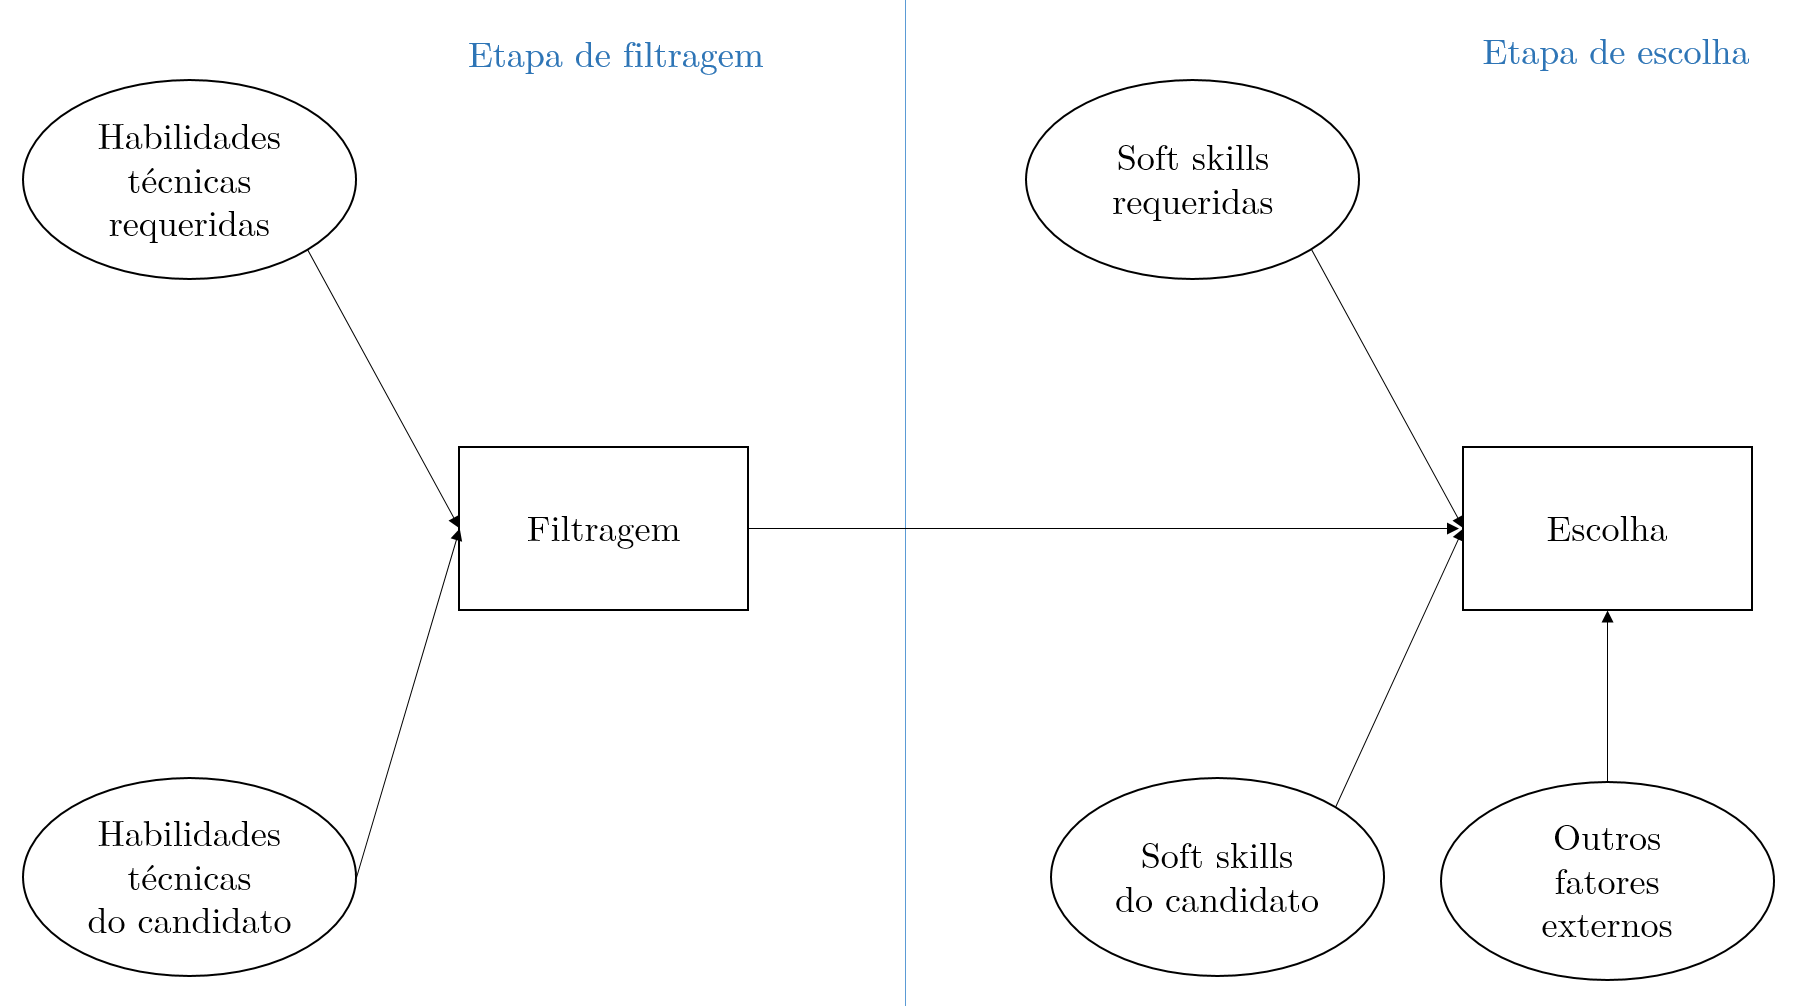
\includegraphics[width=.9\textwidth]{modelocontratacao.png}
\caption{Um modelo de sele��o de pessoal em duas etapas} %\cite{litecky:04}} Precisa citar outra vez na imagem? 
\label{fig:modelocontratacao}
\end{figure}

As habilidades t�cnicas s�o as caracter�sticas b�sicas procuradas em um profissional. Elas funcionam como um filtro. Normalmente, s�o utilizadas para eliminar um candidato que n�o est� apto a um determinado cargo, de acordo com seu curr�culo. Portanto, as habilidades t�cnicas s�o importantes principalmente no processo de recrutamento dos candidatos.

Ap�s o recrutamento, segue-se a fase de contrata��o. Nessa etapa, gerentes e profissionais de recursos humanos costumam dar mais aten��o ao conjunto de habilidades n�o-t�cnicas que o candidato possui. Assim, as soft skills s�o diferenciais nessa etapa, fazendo com que o candidato se destaque entre os demais. Isso demonstra a import�ncia da identifica��o das mesmas e a busca por desenvolver-se como um profissional com um conjunto mais amplo de habilidades, al�m das t�cnicas tradicionais.

Quando consideramos indiv�duos ainda em forma��o educacional, que est�o em busca de est�gio, ou mesmo do primeiro emprego, conhecer e desenvolver soft skills � ainda mais crucial. Esses indiv�duos s�o candidatos com nenhuma, ou pouca, experi�ncia profissional, as soft skills ser�o os valores mais importantes que os mesmos podem apresentar nessa etapa. Elas complementam sua forma��o te�rica e constituem o far�o diferen�a para se tornar o escolhido e ocupar o cargo desejado.

\section{Modelo dos Cinco Fatores}

As teorias de personalidade t�m objetivo de auxiliar no entendimento a respeitos dos interesses, comportamentos e caracter�sticas de cada indiv�duo. Atrav�s dessa �rea da Psicologia, podemos buscar conceitos para entender melhor o que significa cada soft skill, tornando poss�vel identificar como se comporta e quais caracter�sticas s�o expressas por um indiv�duo que possui uma determinada habilidade. Na busca desse conhecimento, nesta se��o explicamos o Modelo dos Cinco Fatores (Five Factor Model - FFM), que � uma teoria da Psicologia sobre personalidade.

O FFM � um modelo para descrever a personalidade atrav�s de uma estrutura de tra�os (traits), em termos de cinco dimens�es b�sicas: Extrovers�o (Extraversion � E), Socializa��o (Agreeableness � A), Realiza��o (Conscientiousness - C), Neuroticismo (Neuroticism - N) e Abertura para experi�ncias (Openness to Experience - O) \cite{mccrae:92}.

Os tra�os de personalidade definidos pelo FFM s�o comumente chamados de ``Big Five��. Cada um dos cinco fatores do modelo representa uma dimens�o dentro da qual um indiv�duo se encontra. Atrav�s de procedimentos de avalia��o, como invent�rios de testes, cada fator � medido para definir os aspectos marcantes da personalidade \cite{costa:85}.

O fator Extrovers�o mostra a tend�ncia por buscar est�mulo na companhia dos outros e no envolvimento com o mundo exterior. Pessoas que pontuam alto neste fator s�o extrovertidas, ou seja, s�o cheias de energia, soci�veis, falantes e entusiasmadas.  Quando uma baixa pontua��o representa esse fator, o indiv�duo � introvertido. Pessoas introvertidas precisam de mais tempo sozinho e buscam mesmo est�mulos que as extrovertidas. Isso n�o significa que eles s�o antissociais, mas que s�o reservados e quietos.

Socializa��o � um fator que descreve o relacionamento interpessoal. Indiv�duos que pontuam alto nesse fator valorizam conviver com os outros. Eles s�o am�veis, acolhedores e compreensivo. Eles tamb�m podem ser generosos e confi�veis. J� os que pontuam baixo, tendem a pensar sobre si mesmo, em vez dos outros, o que significa que eles valorizam o auto-interesse. Normalmente, eles s�o hostis, cr�ticos e briguentos.

O fator Realiza��o descreve pessoas autodisciplinadas. Indiv�duos com alta Realiza��o, apreciam planejamento e organiza��o. Eles s�o persistentes e motivados para atingir seus objetivos. Eles tamb�m prestam aten��o minuciosa aos detalhes, s�o escrupulosos, ambiciosas e decididos. Pelo contr�rio, os indiv�duos com baixa Realiza��o s�o descuidados, desorganizados. Normalmente, se sentem confort�vel com o comportamento espont�neo, decis�es em aberto e tarefas n�o cumpridas.

O fator Neuroticismo indica instabilidade emocional. � a tend�ncia a experimentar emo��es negativas, como raiva, ansiedade ou depress�o. Aqueles que t�m alta pontua��o em Neuroticismo s�o emocionalmente vulner�veis ao estresse. Por outro lado, pontua��es baixas definir pessoas calmas e emocionalmente est�veis.

Abertura para experi�ncias define pessoas interessadas em aprender e explorar novas culturas. Indiv�duos que tendem a apreciar a arte, aventura, ideias incomuns, imagina��o, curiosidade e variedade de experi�ncia. Normalmente, s�o criativos e complexos. Pessoas com baixo pontua��o em Abertura para experi�ncias tendem a ter interesses mais convencionais e tradicionais.

O Modelo dos Cinco Fatores � reconhecido por definir as dimens�es fundamentais da personalidade e por sua aplicabilidade em diversos contextos e culturas. Desde os anos 1960, teoristas da �rea de Psicologia j� buscavam propor um modelo que fosse capaz de definir a personalidade de forma geral e abrangente. No entanto, essa teoria demorou anos para ser estabelecida.

Pesquisas naquela �poca j� reconheciam a ocorr�ncia de cinco fatores \cite{tupes:61} \cite{norman:63}, mas apenas por volta dos anos 1980 come�ou a surgir um consenso a respeito da import�ncia e do estabelecimento deles. Foi quando pesquisadores de diferentes tradi��es desenvolveram estudos a partir da an�lise da linguagem natural e utiliza��o de question�rios de personalidade e observou-se que os cinco fatores mostravam-se convergentes atrav�s de diferentes instrumentos e observadores \cite{mccrae:92}.

Os estudos com base na linguagem natural consistem em uma abordagem l�xica de selecionar os termos de um dicion�rio % \{allport:00}
e agrup�-los em conjuntos de sin�nimos, geralmente utilizando adjetivos para descrever cada dimens�o. Esses adjetivos s�o maneiras de entender as caracter�sticas dos indiv�duos atrav�s de termos que eles mesmos podem avaliar, servindo tamb�m para criar instrumentos de medi��o da personalidade \cite{goldberg:83} \cite{mccrae:85}. Na Tabela \ref{tab:adjetivos} � mostrada, por exemplo, uma lista de adjetivos, originalmente selecionados em ingl�s, para descrever cada dimens�o do FFM, proposta por \cite{john:89} e referida em \cite{mccrae:92}.

\begin{table}[h]
	\centering
		%\begin{tabular}{|c|c|c|}
		\begin{tabular}{|>{\centering\arraybackslash}m{5cm} | >{\centering\arraybackslash}m{4cm} | >{\centering\arraybackslash}m{4cm} |}
		  \hline
			\textbf{Fator} & \textbf{Adjetivos (em ingl�s)} & \textbf{Adjetivos (tradu��o)} \\ \hline
			\textbf{Extrovers�o}	 	& \vtop{\hbox{\strut Active}
														\hbox{\strut Assertive}
														\hbox{\strut Energetic}
														\hbox{\strut Enthusiastic}
														\hbox{\strut Outgoing}
														\hbox{\strut Talkative}}
										& \vtop{\hbox{\strut Ativo}
														\hbox{\strut Assertivo}
														\hbox{\strut Energ�tico}
														\hbox{\strut Entusiasmado}
														\hbox{\strut Soci�vel}
														\hbox{\strut Falante}}
							
			\\ \hline
			\textbf{Socializa��o}	&	\vtop{\hbox{\strut Appreciative}
														\hbox{\strut Forgiving}
														\hbox{\strut Generous}
														\hbox{\strut Kind}
														\hbox{\strut Sympathetic}
														\hbox{\strut Trusting}}
										& \vtop{\hbox{\strut Apreciativo}
														\hbox{\strut Perdoador}
														\hbox{\strut Generoso}
														\hbox{\strut Am�vel}
														\hbox{\strut Compreensivo}
														\hbox{\strut Confiante}}
																					
			\\ \hline
			\textbf{Realiza��o}	&	\vtop{\hbox{\strut Efficient}
														\hbox{\strut Organized}
														\hbox{\strut Planful}
														\hbox{\strut Reliable}
														\hbox{\strut Responsible}
														\hbox{\strut Thorough}}
										& \vtop{\hbox{\strut Eficiente}
														\hbox{\strut Organizado}
														\hbox{\strut Planejado}
														\hbox{\strut Confi�vel}
														\hbox{\strut Respons�vel}
														\hbox{\strut Minucioso}}
			\\ \hline
			\textbf{Neuroticismo}	&	\vtop{\hbox{\strut Anxious}
														\hbox{\strut Self-pitying}
														\hbox{\strut Tense}
														\hbox{\strut Touchy}
														\hbox{\strut Unstable}
														\hbox{\strut Worrying}}
										& \vtop{\hbox{\strut Ansioso}
														\hbox{\strut Auto-piedoso}
														\hbox{\strut Tenso}
														\hbox{\strut Sens�vel}
														\hbox{\strut Inst�vel}
														\hbox{\strut Preocupado}}													
			\\ \hline
			\textbf{Abertura para experi�ncias}	& \vtop{\hbox{\strut Artistic}
														\hbox{\strut Curious}
														\hbox{\strut Imaginative}
														\hbox{\strut Insightful}
														\hbox{\strut Original}
														\hbox{\strut Wide interests}}
										& \vtop{\hbox{\strut Art�stico}
														\hbox{\strut Curioso}
														\hbox{\strut Imaginativo}
														\hbox{\strut Esclarecido}
														\hbox{\strut Original}														
														\hbox{\strut Interesses amplos}}
		\\ \hline
		\end{tabular}
		\caption{Exemplos de adjetivos definindo os Cinco Fatores} %\cite{john:89} \cite{mccrae:92} Precisa citar novamente?
		\label{tab:adjetivos}
\end{table}

%Um desses instrumentos foi proposto por Goldberg \cite{goldberg:83}, atrav�s de uma s�rie de an�lises com base na l�ngua inglesa, a partir da qual 40 pares de adjetivos que foram cuidadosamente selecionados e organizados em 5 grupos de 9 adjetivos cada.
%
%5%%5%%5%%5%%5%%5%%5%%5%%5%%5%%5%%5%%5%%5%%5%%5%%5%%5%%5
%                     Estratégia                       %
%5%%5%%5%%5%%5%%5%%5%%5%%5%%5%%5%%5%%5%%5%%5%%5%%5%%5%%5

\chapter{Estratégia para identificação automática de soft skills}

\label{chap:strategy}

Conhecemos a importância das soft skills para o processo de contração na Subseção \ref{ss-imortance}. Nesse contexto, é comum que as empresas encontrem dificuldades para identificar habilidades de seus candidatos. Isso porque identificar soft skills é uma tarefa que consome tempo, pois é necessário conhecer o indivíduo e seu comportamento durante um determinado período, até ter condições de reconhecer suas habilidades. Para minimizar esse problema, apresentamos uma estratégia que foca no programador de software e visa identificar soft skills de maneira automática.

Dividimos a estratégia para identificaçao automática de soft skills em três passos: (1) Levantamento de soft skills, (2) Conceituação das soft skills, (3) Desenvolvimento de métricas para identificação das soft skills. Podemos observar esses passos na Figura \ref{img:strategy}.

A estratégia é baseada em, inicialmente, entender o significado das soft skills, para então buscar formas de identificá-las.
Durante o primeiro passo, fizemos o levantamento de algumas soft skills do referido papel, tema abordado no Capítulo \ref{chap:research}
O próximo passo é dado no capítulo \ref{chap:concepts}, onde formamos uma base teórica e conceitual a respeito das soft skills. Esse conhecimento é importante para subsidiar o desenvolvimento de métricas para identificação automática.

Abordamos no capítulo \ref{chap:metrics}, o terceiro passo da estratégia, ou seja, o desenvolvimento das métricas para identificação. 



%3%%3%%3%%3%%3%%3%%3%%3%%3%%3%%3%%3%%3%%3%%3%%3%%3%%3%%3
%               Levantamento de soft skills            %
%3%%3%%3%%3%%3%%3%%3%%3%%3%%3%%3%%3%%3%%3%%3%%3%%3%%3%%3

\chapter{Levantamento de soft skills}

\label{chap:research}

Este capítulo é um levantamento bibliográfico baseado em diversos artigos que tratam da importância e da demanda por soft skills no contexto dos profissionais de Tecnologia da Informação (TI) ou de Sistemas de Informação (SI). O objetivo é reconhecer quais são as soft skills necessárias nessa área, focando no papel do programador de software. O resultado desse levantamento é a definição das soft skills com que iremos trabalhar durante o restante desta pesquisa. Portanto, ao final deste capítulo propomos uma lista das soft skills requiridas para o profissional de programação.

Os trabalhos que são referidos neste capítulo abordam o tema das soft skills através quatro abordagens diferentes. Inicialmente, trataremos de estudos que utilizam anúncios de emprego visando identificar a demanda das habilidades profissionais, incluindo soft skills. Há também um estudo que faz uso de entrevistas com membros da faculdade e da indústria para descobrir quais soft skills são consideradas diferenciais de sucesso para um programador. Também apresentamos o que alguns estudos e currículos de cursos de TI e SI ressaltam como soft skills necessárias para a formação do estudante de graduação da área. Por fim, faremos referência a trabalhos que apontam soft skills e as relacionam com teorias da personalidade.

\section{Anúncios de emprego}

Muitos estudos sobre a importância e demanda das soft skills têm sido realizados, por exemplo, Ahmed et al. \cite{ahmed:12} fazem uma análise de 500 anúncios para cargos de TI. Eles se concentram nas soft skills mencionadas nos anúncios para determinar quais estão em alta demanda no setor de desenvolvimento de software. Os anúncios foram coletados a partir de portais de recrutamento online da América do Norte, Europa, Ásia e Austrália. Eles incluiam trabalhos nos cargos de analista de sistemas, designer, programador de computador e testador de software.

No que diz respeito ao papel do programador de computador, os autores encontraram que as habilidades de comunicação estão em alta demanda, solicitada por 90\% dos anúncios. Havia demanda moderada pela habilidade de análise e resolução de problemas e para trabalho independente (demandas entre 52\% e 34\%). Os autores também destacam que os programadores devem ser atento aos detalhes, aprender rápido e ser inovador.

Para Ahmed et al. \cite{ahmed:12}, comunicação é a capacidade de transmitir informação de uma forma que ela seja bem recebida e compreendida. A habilidade de análise e resolução de problemas significa compreender, articular e resolver problemas complexos, tomando decisões sensatas com base nos dados disponíveis. Trabalho independente é poder realizar tarefas com uma supervisão mínima. Atenção a detalhes precisa ser aplicada para compreender o projeto do software e traduzi-lo e código executável. Aprender rápido é ser capaz de aprender novos conceitos e tecnologias em um espaço de tempo relativamente curto. E ser inovador é encontrar soluções novas e criativas.

Outro estudo que utiliza anúncios de empregos, por Lee \cite{lee:05}, coletou 902 anúncios a partir de 230 grandes organizações que fizeram parte da Fortune 500 durante os anos de 2001 e 2003. Lee procurou identificar as hard skills e soft skills que são requeridas para analistas de sistemas. Seus resultados mostraram que as habilidades referentes ao papel do desenvolvedor de software são as mais procuradas nesse setor.

Sobre soft skills, Lee descobriu que comunicação (71,6\%) e habilidades interpessoais (66\%) estavam em alta demanda. A capacidade de trabalhar de forma independente e auto-motivação (29,4\%) estavam em demanda média. Além disso, mais de um quarto dos anúncios de emprego que buscam a habilidade de resolução de problemas.

Kennan et al. \cite{kennan:09} também faz uma análise de 400 anúncios de emprego, dessa vez, o foco está em cargos iniciais da carreira na área de SI. Resultados apontam que nessa fase existe uma alta demanda para a área de desenvolvimento de sistemas (78\%), onde encontramos por exemplo o cargo de programador. Esse estudo ressalta a importância em entender as necessidades e expectativas dos empregadores e suas implicações diretas na formação profissional de graduandos.

Muitas habilidades técnicas e tópicos de conhecimento em computação são mencionadas pelo artigo, no entanto, foram também categorizadas habilidades de comunicação, contabilizando demanda em 73,8\% dos anúncios, e diversas características pessoais, que aparecem em 68,3\% dos anúncios. São listadas soft skills de adaptação, atenção a detalhes, criatividade, aprendizagem rápida, desejo por aprender, organização, resolução de problemas, cooperação, auto-motivação, trabalho independente, etc. 

Embora os estudos acima nos permitiram uma visão geral das soft skills mais importantes para os programadores, há algumas limitações com relação a procurar soft skills em anúncios de emprego. Segundo Litecky \cite{litecky:04}, anúncios de empregos estão focados no processo de recrutamento, ou filtragem de candidados. Como mostrado anteriormente na Figura \ref{fig:modelocontratacao}, essa é a fase onde se procura por habilidades técnicas, nem sempre é comum para os empregadores solicitar soft skills em anúncios de emprego.

Normalmente, as soft skills são investigadas em uma etapa posterior do processo de contratação, na fase de escolha, o que pode ocorrer com base em entrevistas ou recomendações, por exemplo. Isso significa que as soft skills aparecem algumas vezes em anúncios de emprego, mas a demanda real deve ser ainda maior e pode não ser bem representada por eles.

\section{Entrevista com faculdade e indústria}

Através da aplicação de uma abordagem diferente, Sterling e Brinthaupt \cite{sterling:03} entrevistaram membros do corpo docente da faculdade e obtiveram uma lista de critérios de sucesso o programador que trabalha individualmente e para o programador que trabalha em grupo. Em seguida, os membros do corpo docente e da indústria avaliaram a importância dessas características considerando cada caso. Seus resultados apontaram algumas soft skills.

De acordo com membros do corpo docente e da indústria, um programador de sucesso individual tem fortes habilidades de resolução de problemas técnicos, atenção a detalhes, persistência e auto-disciplina para trabalhar sozinho. Um programador de equipe de sucesso é hábil em relações interpessoais, cooperação e comunicação, mostra auto-confiança e consciência.

Esse resultado lista um conjunto de soft skills consideradas relevantes para o sucesso de programadores em diferentes tipos de contextos e sob diferentes pontos de vista. No entanto, o estudo de Sterling e Brinthaupt, e também aqueles que foram referidos anteriormente, não apresentam um conceito exploratório sobre cada soft skills. São dadas apenas breves descrições que não fornecem informação suficiente que pode ser aplicada para identificar essas habilidades em indivíduos.
%Portanto, nosso objetivo é passar por teorias psicológicas para explicar essas características humanas.

\section{Currículo e formação}

Snoke e Underwood \cite{snoke:01} analisam modelos de currículos para programas de graduação em Sistemas de Informação e áreas afins,
como  Guidelines for Undergraduate Degree Programs in Information Systems (IS’97) \cite{is97}
e     Information Systems-Centric Curriculum (ISCC'99) \cite{iscc99},
e um documento que descreve as necessidades da indústria de tecnologia na Austrália,
Australian Computer Society Core Body of Knowledge \cite{acs},
com o objetivo de identificar os principais atributos genéricos que devem ser considerados na formação dos estudantes como futuro profissionais.

Os autores utilizam o termo atributo genéricos para descrever um conjunto de capacidades de um indivíduo. Muitos atributos genéricos apontados pelos autores estão relacionados a habilidades não-técnicas. Assim, identificamos as soft skills resolução de problemas, trabalho independente, apredizagem rápida e comunicação. Apesar dos autores não empregarem esses termos específicos, podemos extraí-los a partir das declarações dos atributos genéricos que são apresentados.

Definir problemas de uma maneira sistemática, analisar, sintetizar e avaliar as várias soluções, considerando a qualidade delas são atributos para a habilidade de resolução de problemas. Confiança em aprender e desempenhar tarefas de forma independente e auto-motivação são atributos para a soft skill trabalho independente. A aprendizagem rápida é uma habilidade de quem possui o atributo de curiosidade sobre tecnologias e capacidade de desenvolver o intelecto em um aprendizado contínuo. A soft skill comunicação pode ser considerada como a habilidade de saber se comunicar escrita e oralmente, trabalhando como parte de um time de forma produtiva e cooperativa.

Os resultados de Snoke e Underwood \cite{snoke:01} foram utilizados em estudos posteriores \cite{snoke:02} e \cite{snoke:03} para comparar currículos de cursos de universidades australianas com os referidos modelos de currículo e com as necessidades da indústria. 
%Esses estudos ressaltam a necessidade dos currículos de cursos de SI e áreas afins serem explícitos em identificar as soft skills dos estudantes e procurar desenvolvê-las durante o curso.
Esses estudos ressaltam que o objetivo da educação superior é equipar os graduandos com os atributos exigidos pelo mercado de trabalho, incluindo aqueles que não são técnicos. Portanto, os educadores precisam ser capazes de identificar as competências de seus alunos e a universidade deve prover uma educação profissional que esteja aliada com as necessidades do mercado.

Em uma versão mais recente do modelo de currículo Guidelines for Undergraduate Degree Programs in Information Systems \cite{is10}, de 2010, o documento aborda principalmente habilidades técnicas a serem desenvolvidas nos estudantes e os perfis de cursos na área de SI. No entanto, é destacada a importância de que todos os cursos precisam desenvolver uma estrutura de pensamento para resolução de problemas, além de fortalecer habilidades de comunicação oral e escrita. Os estudantes também precisam entender que o curso e a profissão exigem persistência, curiosidade, criatividade, etc. O documento ISCC'99 também menciona essas soft skills e suporta esses requisitos.

\section{Mapeamento com teorias da personalidade}
\label{sec:mapeamento}

Em seu artigo, Rehman et al. \cite{rehman:12} atribuem algumas soft skills a profissionais do setor de desenvolvimento de software, abordando os papéis de analista de software, designer, programador, testador e manutenção. De uma forma geral, eles relataram as habilidades de comunicação, habilidades interpessoais, ouvinte ativo, aberto e adaptável a mudanças, inovador, habilidades de organização, aprendizagem rápida, trabalho em equipe, capacidade de trabalhar de forma independente, fortes habilidades analíticas e de resolução de problemas e atenção a detalhes. Especificamente, para os programadores eles indicam as três últimas soft skills como relevantes.

Os autores associaram essas soft skills com o cinco grandes traços da personalidade (Big Five). De acordo com eles, a capacidade de trabalhar de forma independente está relacionada com Extroversão, de uma forma negativa. Fortes habilidades analíticas e de resolução de problemas, com Amabilidade. Atenção a detalhes está relacionada com a Abertura à experiência, também de forma negativa. Esse mapeamento foi feito com base em um estudo anterior, de Capretz e Ahmed \cite{capretz:10}, que também indica as mesmas soft skills.

Dessa forma, a respeito da personalidade do programador, as considerações de Rehman et al. \cite{rehman:12} e recomendações de outros estudos \cite{sodiya:07} \cite{martinez:11}, indicam que esse profissional possui um nível de Extroversão baixo, ou seja, é tipicamente introvertido, se sentindo a vontade em trabalhar sozinho e desenvolver suas tarefas sem necessidade de constante supervisão. Além disso, também possui um alto fator de Amabilidade, sendo alguém que é confiável e cooperativo. O fator Consienciosidade é indicado de forma positiva e Neuroticismo de forma negativa.

A respeito do fator Abertura à experiência, Rehman et al. \cite{rehman:12} e Sodiya et al. \cite{sodiya:07}, recomendam que seu nível seja baixo, por conta da necessidade de prestar atenção a detalhes de implementação e construção do software, que é uma característica oposta a esse fator. Em contrapartida, Martínez et al. \cite{martinez:11} recomenda que o nível de Abertura à experiência seja alto, permitindo características como inovação e criatividade.

Interpretamos que ambas as recomendações são bem-vindas no profissional de programação e com isso podemos mencionar que não existe o programador perfeito, aquele que seja equipado com todas as habilidades possíveis, pois muitas delas podem ir de encontro com a personalidade. Ou seja, cada indivíduo terá os próprios pontos fortes, permitindo a composição de uma equipe de desenvolvimento de software variada, onde cada um poderá se destacar com suas principais habilidades. Vale ressaltar ainda que conhecer o máximo sobre as soft skills e conhecer-se a si próprio é importante para perceber as situações em que será preciso a melhoria de alguma habilidade e o esforço por desenvolvê-la.

Estes estudos foram muito úteis para entender como a personalidade está associada com as soft skills do programador de software, no entanto, eles só apontam três habilidades importantes para esse profissional. Temos a intenção de ampliar essa lista para envolver outras soft skills.

\section{Lista de soft skills}

Com base nas referências encontradas na literatura sobre a demanda e importância das soft skills, resumimos na Tabela \ref{tab:softskills}, as habilidades que escolhemos para trabalhar nesta pesquisa. Como é possível observar, elas foram selecionadas porque apresentaram-se através dos diversos estudos que tratamos durante o levantamento bibliográfico.

\begin{table*}[h]
\footnotesize
\caption{\small Soft skills apontadas na literatura para profissionais da área de TI} 
\addtolength{\tabcolsep}{-3.5pt}
\centering

		\begin{tabular}{|p{7cm}|c|c|c|c|c|c|c|c|c|}\hline
		
        \multicolumn{1}{|r|}{\bf Referências} & 1 & 2 & 3 & 4 & 5 & 6 & 7 & 8 & 9 \\\hline
				
{\bf Comunicação} & \ding{51} & \ding{51} & \ding{51} & \ding{51} & \ding{51} & \ding{51} & \ding{51} & \ding{51} & \ding{51}
\\\hline
{\bf Trabalho independente} & \ding{51} & \ding{51} & \ding{51} & \ding{51} & \ding{51} & \ding{51} & \ding{51} & & 
\\\hline
{\bf Atenção a detalhes}  & \ding{51} & \ding{51} &  & \ding{51} & \ding{51} & \ding{51} & & &
\\\hline
{\bf Análise e resolução de problemas} & \ding{51} & \ding{51} & \ding{51} & \ding{51} & \ding{51} & \ding{51} & \ding{51}  & \ding{51} & \ding{51}
\\\hline
{\bf Persistência} &  & \ding{51} &  &  &  &  &  & \ding{51} & \ding{51} 
\\\hline
{\bf Aprendizagem rápida} & \ding{51} &  &  & \ding{51} & \ding{51} & \ding{51} & \ding{51} & &
\\\hline

     \end{tabular}
		\label{tab:softskills}
		\fonte{1 - \cite{ahmed:12}; 2 - \cite{sterling:03}; 3 - \cite{lee:05}; 4 - \cite{kennan:09}; 
			5 - \cite{rehman:12}; 6 - \cite{capretz:10}; 7 - \cite{snoke:01}; 8 - \cite{iscc99}; 9 - \cite{is10}}
\end{table*}

Dessa maneira, damos destaque para uma lista de seis soft skills que afirmamos ser relevantes para a qualificação profissional para os programadores de software: Análise e resolução de problemas, Atenção a detalhes, Aprendizagem rápida, Persistência, Comunicação, Trabalho independente.

Essa lista de soft skills envolve diferenciais para integração, permanência e crescimento do programador como profissional. No entanto, é preciso ressaltar que ela não tem objetivo de ser exaustiva, e não o é. As soft skills importantes para qualquer profissional podem ser listada, mas é sempre possível considerar mais alguma. Portanto, para fins desta pesquisa, definimos a lista proposta neste capítulo como escopo.

%Desse ponto em diante, iremos explicar porque cada uma dessas soft skills é importante e como se aplicam no ambiente de trabalho do programador. Além disso, propomos um conceito sobre cada uma delas, através de um mapeamento com o Modelo dos Cinco Fatores. 

%4%%4%%4%%4%%4%%4%%4%%4%%4%%4%%4%%4%%4%%4%%4%%4%%4%%4%%4
%             Conceitua��o das soft skills             %
%4%%4%%4%%4%%4%%4%%4%%4%%4%%4%%4%%4%%4%%4%%4%%4%%4%%4%%4

\chapter{Conceitua��o das soft skills}

Neste cap�tulo, explicamos a import�ncia das soft skills que escolhemos para esta pesquisa, as quais foram listadas no Cap�tulo \ref{cap:research}. Aqui discutimos suas aplica��es na profiss�o do programador de software e propomos um mapeamento com os tra�os de personalidade descritos pelo Modelo dos Cinco Fatores. O objetivo deste cap�tulo � esclarecer o significado de cada soft skill e encontrar informa��es suficientes para desenvolver formas de identific�-las automaticamente.

\section{An�lise e resolu��o de problemas}

\section{Aten��o aos detalhes}

\section{Aprendizagem r�pida}

\section{Persist�ncia}

\section{Comunica��o}


%5%%5%%5%%5%%5%%5%%5%%5%%5%%5%%5%%5%%5%%5%%5%%5%%5%%5%%5
%                     Estratégia                       %
%5%%5%%5%%5%%5%%5%%5%%5%%5%%5%%5%%5%%5%%5%%5%%5%%5%%5%%5

\chapter{Estratégia para identificação automática das soft skills}

\label{chap:metrics}

Conhecemos a importância das soft skills para o processo de contratação na Subseção \ref{subsec:ss-importance}. Nesse contexto, é comum que as empresas encontrem dificuldades para identificar habilidades de seus candidatos. Isso porque identificar soft skills é uma tarefa que consome tempo, pois é necessário conhecer o indivíduo e seu comportamento durante um determinado período, até ter condições de reconhecer suas habilidades. Para minimizar esse problema, apresentamos uma estratégia que foca no papel do programador de software e visa identificar soft skills de maneira automática.

%Dividimos a estratégia para identificaçao automática de soft skills em três passos: (1) Levantamento de soft skills, (2) Conceituação das soft skills, (3) Desenvolvimento de métricas para identificação das soft skills. Podemos observar esses passos na Figura \ref{fig:estrategia}.

%\begin{figure}[h*]
%\centering
%\caption{\small Estratégia para identificaçao automática de soft skills} 
%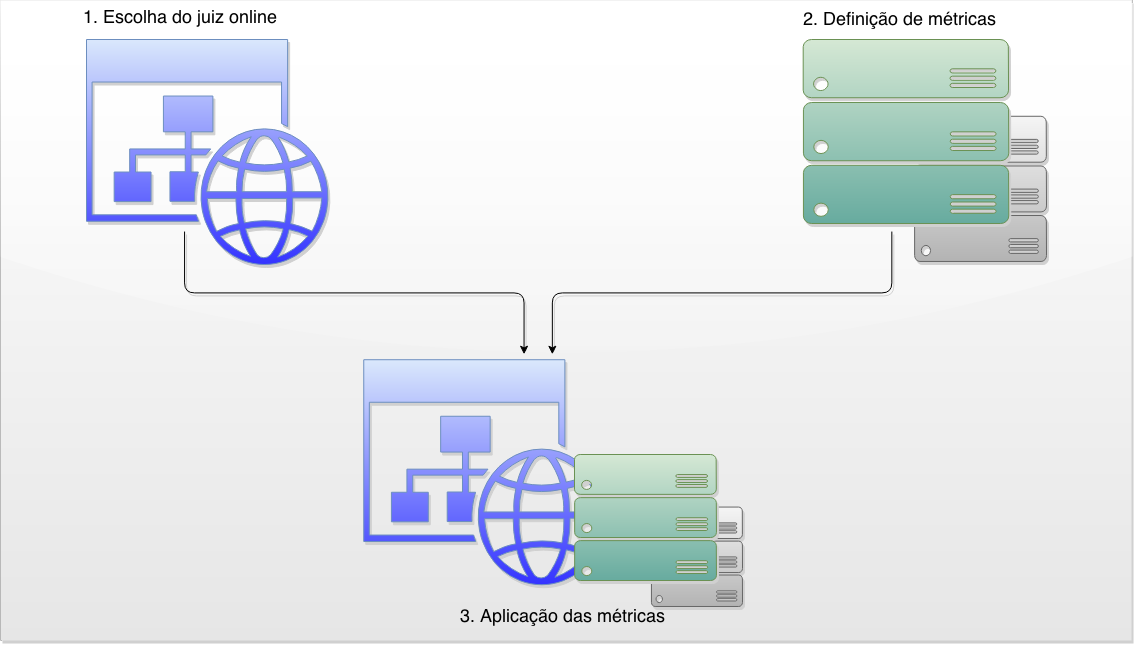
\includegraphics[width=.9\textwidth]{estrategia.png}
%\label{fig:estrategia}
%\end{figure}


Essa estratégia está baseada, inicialmente, em entender o significado das soft skills, para então buscar formas de identificá-las.
Até este ponto, fizemos o levantamento de algumas soft skills do referido papel, tema abordado no Capítulo \ref{chap:research}. Em seguida, no Capítulo \ref{chap:concepts}, formamos uma base teórica e conceitual a respeito das soft skills.
Agora iremos detalhar a estratégia em si.

Para atingir o objetivo de identificar soft skills de maneira automática, levamos em consideração alguns pontos. Primeiramente, sabemos que é preciso conhecer o comportamendo do indivíduo para reconhecer suas habilidades. Portanto, propomos que, para identificar as soft skills de um programador, é necessário observá-lo em suas atividades de programação. Além disso, como a identificação deve ocorrer automaticamente, precisamos utilizar um ambiente que possibilite a coleta automática de informações a respeito do comportamento de um programador.

Assim, nossa estratégia consiste no desenvolvimento de métricas que atribuem uma pontuação para cada soft skill de um programador. O ambiente em que podemos coletar essas métricas automaticamente é um juiz online, sistema no qual os usuários praticam atividades de programação. Esse tipo de sistema possui uma base de dados que guarda as interações dos usuários, as quais podem ser analisadas a partir das referidas métricas, representando uma alternativa para identificação das soft skills.

%Then, we propose to use the past interaction of the student to identify soft skills by analyzing their previous interaction history based on their concepts and making use of metrics that can represent an alternative to know a person. As a source for this metrics, one might rely on online programming tools, since these systems allow the evaluation of its user's behavior. A popular category of this kind of system is the online judges. In subsection 3.1, we present the online judge system that we use in this paper.

%Portanto, dividimos a estratégia para identificaçao automática de soft skills em três passos: (1) Escolha de um juiz online, (2) Desenvolvimento de métricas, (3) Coleta de métricas utilizando a base de dados do juiz online. Podemos observar esses passos na Figura \ref{img:strategy}.

Na Seção \ref{sec:huxley}, tratamos das principais características de um juiz online e apresentamos o sistema que adotamos nesta dissertação. Adicionalmente, na Seção \ref{sec:metrics}, propomos as métricas para identificação de soft skills nos usuários de um juiz online.

\section{Juiz online} 
\label{sec:huxley}

O juiz online é um sistema que disponibiliza um conjunto de problemas de programação a serem resolvidos através da criação e codificação de algoritmos. O usuário do sistema pode acessar os problemas e submeter soluções para os mesmos. O juiz online avalia essas submissões testando-a de acordo com um conjunto de casos de teste predefinidos. Se a submissão passa por todos os casos de teste, o sistema a avalia como correta. Caso contrário, o sistema avalia a submissão de acordo com o tipo de erro, por exemplo, resposta errada, erro de compilação, tempo limite excedido, etc.

Nesse contexto, ao interagir com o sistema, os programadores geram informação que pode ser coletada e aplicada a métricas, visando identificar soft skills automaticamente. Neste estudo, utilizamos para este fim, o juiz online Huxley \cite{paes:13}. O sistema está disponível para acesso online através do endereço \textit{www.thehuxley.com}.

A maioria dos usuários do juiz online Huxley são estudantes de programação. O Huxley oferece uma base com mais de 450 problemas de programação, organizados por níveis de dificuldade (um a 10) e por assunto: entrada formatada, repetição, string, ordenação, acumulador, múltiplas entradas, decisão, array bidimensional e estrutura de dados.

A base de dados do Huxley também armazena todas as submissões de seus usuários. Atualmente, existem cerca de 150,000 submissões, corrigidas de acordo com os tipos de avaliação do Huxley: Correta, Resposta errada, Erro de apresentação, Erro de compilação, Resposta vazia, Erro de execução, Tempo limite excedido, Nome errado de arquivo. 
Nos casos quando a submissão não é avaliada como Correta, o Huxley oferece dicas ao usuário para auxiliá-lo a resolver o problema. 

O Huxley é utilizado em diversas universidades e faculdades com cursos na área de computação, inclusive na Universidade Federal de Alagoas, onde é ferramenta para avaliação e incentivo à prática de programação, empregada na disciplina inicial de Programação 1, no cursos de Ciência da computação e Engenharia da Computação.

No Huxley, cada usuário pode desenvolver seu próprio ritmo na prática de programação. Não existe uma ordem para resolução dos problemas, deixando o usuário livre para interagir com o sistema de acordo com os níveis dos mesmos. A cada submissão correta, o usuário recebe uma pontuação para incentivá-lo, no entanto, ele não é penalizad caso tenha submissão avaliada como errada. Os usuários também são ordenados de acordo com suas pontuações, compondo um ranking de programadores, chamado de TopCoder.

Neste estudo, escolhemos utilizar o juiz online Huxley porque ele oferece funcionalidades suficientes para aplicação das métricas de indentificação das soft skills do programador de software. Sua base de dados será a fonte para coleta dessas métricas. Além disso, temos acesso ao time de desenvolvimento e a alguns usuários do sistema, a saber, estudantes de programação da Universidade Federal de Alagoas.

Como exemplo de como podemos utilizar o Huxley para coletar métricas, podemos analisar os níveis de problemas que cada usuário resolve, o que nos oferece informações a respeito das habilidades de resolução e análise de problemas. Outro exemplo, como o sistema não penaliza submissões erradas, o usuário é incentivado a tentar outras vezes até conseguir, o que nos traz informações para verificar a habilidade de persistência.

\section{Métricas} 
\label{sec:metrics}

Como dito anteriormente, as métricas que propomos são alternativas que auxiliam na medição do nível de cada soft skill em um indíviduo de acordo com seu comportamento em atividades de programação. As soft skills que visamos medir são: Análise e resolução de problemas, Atenção a detalhes, Aprendizagem rápida, Persistência, Comunicação, Trabalho independente.

Cada uma das métricas aqui propostas avaliam uma soft skill com valor no intervalo de zero a 100. Quanto maior o valor resultante da métrica para uma determinada soft skill, significa que o indíviduo possui essa habilidade mais desenvolvida. Dessa forma, se uma soft skill for medida em zero, significa que o indivíduo não possui essa habilidade. Se o valor for 100, ele possui a habilidade de uma maneira ótima. Escolhemos avaliar cada soft skill em um intervalo de zero a 100, para que fosse possível ordenar os resultados dos indivíduos e conhecer suas principais habilidades, bem como, as que precisam de melhoria.

A seguir, iremos apresentar as métricas para identificação de soft skills dos usuários do Huxley. Embora essas métricas tenham sido aplicadas a um sistema específico, elas podem ser também empregadas em sistemas similares, ou seja, podem ser adaptadas para outros juizes online.

\subsection{Análise e resolução de problemas}

Para desenvolver as métricas de identificação automática dessas habilidades em um indivíduo, utilizamos sua interação com sistema Huxley. Aqui propomos duas métricas, uma está relacionada com a habilidade de Resolução de problemas. A outra, está relacionada com Análise de problemas.

A métrica Resolução de problemas leva em conta a quantidade de soluções, ou seja, quantas submissões um usuário envia ao Huxley. Quanto mais um usuário envia submissões ao sistema, mais ele demonstra gostar de resolver problemas de programação. Por exemplo, dependendo do nível de dificuldade do problema, o usuário pode ter que apresentar diversas submissões ao sistema para conseguir resolvê-lo. No entanto, observe que isso não é necessariamente uma coisa ruim, por conta do processo de aprendizagem e pratica de programação, que é a essência de Huxley. Enviar muitas submissões significa que o usuário está de alguma forma estudando e praticando programação continuamente.

Considere que $SUBMISSIONS$ é o número de submissões que o usuário enviou para o Huxley. 
Para fazer com que a métrica de Resolução de problemas seja avaliada de zero a 100, temos que tomar um valor de referência. Este valor de referência é o número máximo de submissões de um usuário já enviou ao Huxley, chame de $SUBMISSIONS_{MAX}$. Assim, a métrica é calculada da seguinte forma:

\begin{equation} \label{m:resolucao}
\mbox{Resolução de problemas } = \frac{SUBMISSIONS}{SUBMISSIONS_{MAX}} * 100
\end{equation}

Portanto, o usuário que enviou mais soluções para o sistema vai pontuar 100 na habilidade de Resolução de problemas. A pontuação dos demais usuários será calculada relativamente a esse número máximo de submissões.

No entanto, quando consideramos apenas o número de submissões isoladamente, um elevado número de submissões erradas também pode significar que o aluno não está analisando muito bem o problema antes de tentar outras vezes. Desta forma, propomos a métrica de Análise de problemas, considerando agora o número de submissões corretas, levando em consideração quantos problemas o usuário foi capaz de resolver e os níveis desses problemas.

Para cada apresentação correta, o usuário do Huxley recebe uma pontuação dependendo do nível do problema que esta submissão responde. Por exemplo, quando um usuário resolve o problema de nível 1, ela ganha um ponto. Da mesma forma, se o problema é o nível 2, ele recebe 2 pontos. A pontuação máxima é de 10, para submissões corretas de problemas nível 10.

Agora, dado que $CORRECT_{SCORE}$ é a soma da pontuação das submissões corretas do usuário. Além disso, dado que $SUBMISSIONS_{SCORE}$ é a soma da pontuação de todas as submissões do usuário. A métrica para de Análise de problemas é:

\begin{equation} \label{m:analise}
\mbox{Análise de problemas } = \frac{CORRECT_{SCORE}}{SUBMISSIONS_{SCORE}} * 100
\end{equation}

Note que a métrica dessa soft skill pode ser avaliada entre zero e 100. Quanto mais o usuário envia submissões corretas, sua pontuação tende a 100. Caso contrário, se o usuário envia muitas submissões erradas, sua pontuação tende a zero.

\subsection{Atenção a detalhes}

Um indivíduo que presta atenção a capaz de utilizar de forma completa todos os recursos disponíveis para realizar suas atividades. No contexto de um juiz online, o usuário atento precisa conhecer bem o sistema e saber como tirar proveito de todas as suas funcionalidades.

Por exemplo, para cada problema do Huxley existe um exemplo de entrada e saída na descrição do problema. Esta entrada e saída é o primeiro caso de teste que avalia cada submissão. Um usuário atento deve sempre observar cuidadosamente essa funcionalidade, para que escrever sua submissão seguindo o exemplo. Com isso, ele evita apresentar soluções que falham no primeiro caso de teste.

Além disso, um usuário atento não apresenta submissões que causam erros de compilação, porque ele conhece os detalhes de sintaxe da linguagem que utiliza, e provavelmente testou seu código antes de submetê-lo.

Dessa forma, para identificar se um usuário possui a soft skill Atenção a detalhes, podemos analisar esses pontos. Para um usuário, seja $IO_{ERROR}$ o número de submissões que falham no primeiro caso de teste, e $SYNTAX_{ERROR}$ o número de submissões que foram avaliadas com erros de compilação. Seja ainda $SUBMISSIONS$ o número total de submissões por parte do usuário ao sistema. Definimos a métrica como se segue:

\begin{equation} \label{m:atencao}
\mbox{Atenção aos detalhes } = \left(1 - \frac {IO_{ERROR} + SYNTAX_{ERROR}}{SUBMISSIONS}\right) * 100
\end{equation}

Note que, se o usuário sempre envia submissões com erros de sintaxe ou erra no exemplo de entrada/saída, o quociente 
$\frac {IO_{ERROR} + SYNTAX_{ERROR}}{SUBMISSIONS}$ vale um. Portanto, a medida de Atenção a detalhes torna-se zero.
No entanto, se ele sempre está atento para evitar esses erros simples, o quociente passa a valer zero e a métrica de Atenção aos detalhes é avaliada em 100.

\subsection{Aprendizagem rápida}

Para identificar Aprendizagem rápida, é necessário estabelecer um critério de comparação, uma vez que essa soft skill diz respeita a capacidade de aprender em um tempo relativamente curto. No juiz online Huxley, os usuários estão agrupados por turma, equivalente a classe no curso de programação de que fazem parte. Para propor a métrica de aprendizagem rápida, estamos considerando a turma como fator comparativo.

No cálculo dessa métrica, primeiramente, determinamos para cada usuário do Huxley sua velocidade para resolver problemas, ou seja poara obter pontuação em submissões corretas. Tomamos a soma da pontuação das submissões corretas do usuário, $CORRECT_{score}$, para cada dia considerando dois dias diferentes e sequenciais ($DAY_0$ e $DAY_f$). Assim, a velocidade $SPEED$ para resolver problemas é dada por:

\begin{equation} \label{m:velocidade}
SPEED = \frac {CORRECT_{score} \mbox{ em } DAY_f - CORRECT_{score} \mbox{ em } DAY_0 }
              { \mbox{ Dias entre } DAY_0 \mbox{ e } DAY_f }
\end{equation}

% Continuamos cálculo da velocidade em uma janela de 6 meses. Depois disso, calcula-se a variação de velocidade para obter o ACC, o que vai significar a aceleração média de aprendizagem.

Precisamos ainda tomar um valor de referência para avaliar a métrica de Aprendizagem rápida entre zero e 100. Este valor de referência é a velocidade máxima $SPEED_{MAX}$ obtida na turma. Em seguida, a métrica para esta soft skill é calculada da seguinte forma:

\begin{equation} \label{m:aprendizagem}
\mbox{Aprendizagem rápida } = \frac{SPEED}{SPEED_{MAX}} * 100
\end{equation}

com uma regra de três, tendo como referência a maior velocidade da turma que o usuário pertence. Assim, o usuário que aprendeu mais rápido em cada grupo vai marcar 100. A pontuação dos demais será calculado relativamente a essa.

\subsection{Persistência}

Propomos a métrica de Persistência com base na quantidade de vezes que o usuário continua tentando resolver um problema. Quanto mais o usuário envia submissões, mais ele demonstra estar praticando continuamente. Mesmo que ele não está obtendo uma solução correta, está se esforçando e, eventualmente, irá conseguir acertar. Esse comportamento está relacionado a persitência diante de adversidade na resolução do problema.

% Além disso, mesmo depois de uma solução correta, o usuário pode tentar submeter novamente, tentando melhorar o algoritmo. Esse tipo de comportamento também demonstra persistência.

Para medir a soft skill Persistência, considere que $CORRECT_{PROBLEMS}$ é número de problemas resolvidos por um usuário, excluindo os problemas que foram resolvidos corretamente na primeira tentativa. Considere ainda que $PROBLEMS$ é o número total de problemas que o usuário já tentou resolver, também sem contar os que foram acertados na primeira tentativa. Recomendamos que não contar com esses problemas, porque como a solução foi obtida com apenas uma tentativa, o usuário não teve necessidade de demonstrar um comportamento persistente.

Aqui poderíamos dividir $CORRECT_{PROBLEMS}$ por $PROBLEMS$ para obter uma medida de Persistência.
No entanto, é interessante também levar em conta aqueles problemas que o usuário tentou várias vezes. Os quais, mesmo que ele que ainda não tenha obtido uma solução, pelo menos, tenha se esforçado para resolver. Então, calculamos a média de tentativas feitas pelos usuários até acertar cada problema do Huxley.

A partir disso, chame $EFFORT_{PROBLEMS}$ o número de problemas não resolvidos, mas que o número de tentativas foi acima da média de tentativas para cada um desses problemas. 
Por exemplo, se a média de tentativas até acertar o problema $\#1$ é $4$, e para o problema $\#2$ é $10$. Se o usuário tentou $5$ vezes, mais ainda não acertou o problema $\#1$, e o problema $\#2$, tentou $8$ vezes. O problema $\#1$ será contado em $EFFORT_{PROBLEMS}$. Mas o problema $\#2$ não será, pois o número de tentativas foi menor que a média de tentativas para resolver o problema.

Assim, propomos a métrica:

\begin{equation} \label{m:persistencia}
\mbox{Persistência } = \frac{ CORRECT_{PROBLEMS} + EFFORT_{PROBLEMS} }{ PROBLEMS } * 100
\end{equation}

Para alcançar a pontuação máxima em Persistência, que é 100, o usuário não deve deixar que problemas sem uma solução correta, ou pelo menos ele tem que se esforçar, acima da média, para resolvê-los. Por outro lado, se um usuário deixa todos os problemas com soluções incorretas, sua pontuação de persistência é zero.

\subsection{Comunicação}

No contexto de programação, propomos que alguém que tem habilidades de Comunicação escreve documentação de seus artefatos, costumando, por exemplo, comentar seus códigos-fonte. Além disso, no contexto de um sistema de juiz online, o indivíduo utiliza recursos de bate-papo para entrar em contato com outros usuários e participa em fóruns como objetivo ampliar sua comunidade.

Seria interessante fazer uso de todas essas características para definir a métrica de identificação da soft skill Comunicação. No entanto, o Huxley não possui as funcionalidade de bate-papo ou fórum. Por isso, optamos por apenas considerar os comentários de código-fonte.

Para um usuário, tomamos os arquivos de código-fonte de suas submissões corretas. Para cada arquivo selecionada, verificamos se ele possui comentários nas linhas de código. Seja $COMMENTED$ a quantidade de arquivos de código-fonte que tenham pelo menos um comentário, e $FILES$ o número de arquivos analisados. A métrica de Comunicação é definido como segue:

\begin{equation} \label{m:comunicacao}
\mbox{Comunicação } = \frac{ COMMENTED }{ FILES } * 100
\end{equation}

Note que, o valor da métrica está entre 0 e 100. Se o usuário costuma comentar seus arquivos de código-fonte, sua pontuação em Comunicação tende a 100. Por outro lado, se ela nunca comenta os códigos, sua pontuação em Comunicação é zero.

\subsection{Trabalho independente}

Sabemos que se alguém pode resolver problemas de programação com o mínimo de supervisão e não sente necessidade de pedir ajuda, mesmo diante de problemas de níveis altos de dificuldade, esse indivíduo sabe trabalhar de forma independente.

O Huxley oferece duas maneiras de pedir ajuda. Caso o usuário esteja com dúvidas diante de ua submissão, ele pode deixar uma pergunta no sistema, a qual será ao professor responsável ou monitores de disciplina. O professor ou monitor, então, responde a dúvida escrevendo comentários para auxiliar na resolução do problema. Outra forma de pedir juda é quando um usuário tem uma submissão que não foi avaliada como correta. Nesse casos, o sistema oferece a oportunidade de ler uma dica, que é um comentário escrito pelo autor do problema informando qual foi o erro ou como obter a solução certa. No entanto, ler essa dica é opcional.

Seja $TIPS$ o número de dicas que um usuário aceita visualizar e $HELPS$ número de submissão em que o usuário pediu e recebeu comentários de ajuda. Chame $SUBMISSIONS$ o número de submissões do usuário. A métrica que representa Trabalho independentemente é dada por:

\begin{equation} \label{m:independente}
\mbox{Trabalho independente } = \left(1 - \frac {TIPS + HELP}{SUBMISSIONS}\right) * 100
\end{equation}

Observe que, se um usuário pedir dicas ou ajuda para todas as suas apresentações a TIP quociente + Ajuda / SUBS serão valor como 1, levando Trabalho marcar de forma independente a 0. O oposto disso é quando um usuário nunca pedir ajuda ou dicas. Em seguida, trabalhar de forma independente pontuação é 100.

Observe que, se o usuário sempre visualiza dicas ou envia dúvidas e recebe ajuda para resolver os problemas, o quociente 
$\frac {TIPS + HELP}{SUBMISSIONS}$ vale um. Portanto, a medida de Trabalho independente torna-se zero.
O oposto disso é quando o usuário não necessita de ajuda ou dicas, de forma que o quociente passa a valer zero e a métrica de Trabalho independente é avaliada em 100.

\section{Coleta de métricas utilizando a base de dados do juiz online}

Para ilustrar a aplicação das métricas propostas neste Capítulo, observe a Tabela \ref{tab:dadosmetricas}. Nela mostramos os dados que coletamos para calcular as métricas de cada soft skill. Por motivos de privacidade, estamos apresentando dados de um usuário fictício, chamado John Smith.

\begin{table*}[h]
\footnotesize
\caption{\small Dados que coletados para calcular as métricas} 
\addtolength{\tabcolsep}{-3.5pt}
\renewcommand{\arraystretch}{1.5} 
\centering

		\begin{tabular}{|p{9cm}|l|c|}\hline
		
        Informação & Variável & Dado \\\hline\hline
				
				\multicolumn{3}{|c|}{\textbf{Sobre o Huxley}} \\\hline
								
				Número máximo de submissões & $ SUBMISSIONS_{MAX}$	& 713 \\\hline\hline
				
				
				\multicolumn{3}{|c|}{\textbf{Sobre a turma de John Smith}} \\\hline
					
				Velocidade máxima de pontuação &  $ SPEED_{MAX}$ 	& 13,6 pontos/dia \\\hline\hline
				
				
				\multicolumn{3}{|c|}{\textbf{Sobre John Smith}} \\\hline
				
				Número de submissões 												& $ SUBMISSIONS$ & 647		\\\hline
				Soma das pontuações das submissões 					& $ SUBMISSIONS_{SCORE}$ & 2814	\\\hline
				%Número de submissões corretas 							& & 226		\\\hline
				Soma das pontuações das submissões corretas & $ CORRECT_{SCORE}$		 & 681 	\\\hline
				
				Número de submissões com erro de sintaxe											& $ IO_{ERROR}$				& 9 		\\\hline
				Número de submissões com erro no exemplo de entrada e saída		& $ SYNTAX_{ERROR}$		& 86 		\\\hline
				
				Velocidade de pontuação																				& $ SPEED$						& 13,6 pontos/dia 	\\\hline
				
				Problemas tentados,
				sem contar os resolvidos na primeira tentativa				& $ PROBLEMS$ 								& 92		\\\hline
				Problemas resolvidos,
				sem contar os resolvidos na primeira tentativa				& $ CORRECT_{PROBLEMS}$ 			& 52		\\\hline
				Problemas não resolvidos,
				mas tentados por um número de vezes acima da média		& $ EFFORT_{PROBLEMS}$ 				& 10		\\\hline
				
				Número de códigos-fonte analisados										& $ FILES$ 										& 647		\\\hline
				Número de códigos-fonte comentados										& $ COMMENTED$ 								& 114		\\\hline
				
				Número de submissões com dica													& $ TIPS$ 										& 35		\\\hline
				Número de submissões com ajuda												& $ HELP$ 										& 4			\\\hline
				
					
     \end{tabular}
		\label{tab:dadosmetricas}
		%\fonte{}
\end{table*}

A partir dos dados coletados da base do Huxley, podemos então aplicar as métricas para identificar o nível de cada soft skill do usuário John Smith. Observe o exemplo dessa aplicação na Tabela \ref{tab:metricas}.

\begin{table*}[h]
\footnotesize
\caption{\small Métricas para identificar o nível das softs skills}
\addtolength{\tabcolsep}{-3.5pt}
\renewcommand{\arraystretch}{1.7} 
\centering

		\begin{tabular}{|p{4cm}|p{7cm}|p{3cm}|c|}\hline
		
        \textbf{Soft skill} & \textbf{Métrica} & \multicolumn{2}{c|}{\textbf{Valor}} \\\hline
													
				Resolução de problemas & $\frac{SUBMISSIONS}{SUBMISSIONS_{MAX}} * 100$
															 & $\frac{647}{713} * 100$ & 90,74 \\\hline
				
				Análise de problemas & $\frac{CORRECT_{SCORE}}{SUBMISSIONS_{SCORE}} * 100$
														 & $\frac{681}{2814} * 100$ & 24,20 \\\hline
				
				Atenção a detalhes & $\left(1 - \frac {IO_{ERROR} + SYNTAX_{ERROR}}{SUBMISSIONS}\right) * 100$
													 & $\left(1 - \frac {9 + 86}{647}\right) * 100$ & 85,32 \\\hline
				
				Aprendizagem rápida & $\frac{SPEED}{SPEED_{MAX}} * 100$
														& $\frac{13,6}{13,6} * 100$ & 100,00 \\\hline
				
				Persistência & $\frac{CORRECT_{PROBLEMS} + EFFORT_{PROBLEMS}}{PROBLEMS} * 100$
										 & $\frac{52 + 10}{92} * 100$ & 67,39 \\\hline
				
				Comunicação & $\frac{COMMENTED}{FILES} * 100$
										& $\frac{114}{647} * 100$ & 17,62	\\\hline
				
				Trabalho independente & $\left(1 - \frac {TIPS + HELP}{SUBMISSIONS}\right) * 100$
															& $\left(1 - \frac {35 + 4}{197}\right) * 100$ & 80,20 \\\hline
													
     \end{tabular}
		\label{tab:metricas}
		%\fonte{}
\end{table*}

%6%%6%%6%%6%%6%%6%%6%%6%%6%%6%%6%%6%%6%%6%%6%%6%%6%%6%%6
%                     Validação                        %
%6%%6%%6%%6%%6%%6%%6%%6%%6%%6%%6%%6%%6%%6%%6%%6%%6%%6%%6

\chapter{Estudo de validação}

\label{chap:evaluation}

Para avaliar a estratégia que apresentamos no Capítulo \ref{chap:metrics}, conduzimos um estudo empírico a fim de analisar se as métricas que propomos são capazes de identificar as soft skills dos indivíduos que utilizam o juiz online Huxley.

Neste estudo, consideramos a relação que existe entre as soft skills e os fatores de personalidade que discutimos no Capítulo \ref{chap:concepts}. Propomos comparar se o resultado obtido através da aplicação das métricas identificam as soft skills associadas aos fatores de personalidade de um indivíduo. Para isso, coletamos as métricas que detalhamos na Seção \ref{sec:metrics} em um grupo de usuários do Huxley. Em seguida, os convidamos para responder um breve questionário a respeito de personalidade, com o objetivo de comparar os resultados. 

Para explicar o estudo de validação, apresentamos os participantes e o material na Seção \ref{sec:participantes} e Seção \ref{sec:material}, respectivamente. Na Seção \ref{sec:procedimento}, detalhamos o procedimento que seguimos durante a avaliação das métricas para identificação de soft skills. Na Seção \ref{sec:ameacas}, discutimos as principais ameaças à validade e como as contornamos.

\section{Participantes}
\label{sec:participantes}

Os participantes do estudo de validação são usuários do Huxley e estudantes matriculados nas disciplinas de Programação 1 dos cursos de Ciência da Computação e Engenharia da Computação, na Universidade Federal de Alagoas. A Tabela \ref{tab:participantes} distribui o número de participantes por semestre e curso:

\begin{table*}[ht]
\footnotesize
\caption{\small Participantes}
\addtolength{\tabcolsep}{-3.5pt}
\renewcommand{\arraystretch}{1.4} 
\centering

\begin{tabular}{|c|c|c|}
\hline
\textbf{Semestre} & \textbf{Curso} 		& 	\textbf{Número de estudantes matriculados} \\ \hline
2014.1 & Ciência da Computação 		 		& 	33 		\\ \hline
2014.1 & Engenharia da Computação 		& 	23 		\\ \hline
\multicolumn{2}{|c|}{\textbf{Total}} 	&		56 		\\ \hline
\end{tabular}

\label{tab:participantes}
\end{table*}

A disciplina de Programação 1, em ambos os cursos, tem o objetivo de capacitar o estudante em assuntos que envolvem análise e resolução de problemas, desenvolvimento de algoritmos utilizando linguagem de programação, estruturação de programas, noções de tipos e estrutura elementares de dados e conceitos de recursão \cite{cc:projeto, ec:projeto}. Atualmente, a linguagem de programação C é utilizada durante a disciplina.

Com o objetivo de estimular os estudantes, os professores incentivam a utilização do Huxley para prática e aprendizagem de programação de forma espontânea. Todos os problemas de programação contidos no sistema estão disponíveis para submissão a qualquer momento, ou seja, os alunos podem acessar o Huxley para atividades extraclasse e estabelecer seu próprio ritmo de estudos.

As aulas de Programação 1 aconteceram em um laboratório de informática. Durante as aulas, os professores utilizaram problemas do Huxley para resolvê-los como exercício. O uso do juiz online foi obrigatório apenas para atividades avaliativas, compondo parcialmente a nota de desempenho na disciplina.

No final do período de aulas, o banco de dados do Huxley guardava as interações dos usuários participantes com relação a suas atividades de programação durante a disciplina, as quais foram analisadas de acordo com as métricas para identificação de soft skills.
Nesse mesmo tempo,  
tivemos acesso presencial às turmas, para que os participantes respondessem o questionário a respeito da personalidade, de maneira que a medição das soft skills e as respostas dos questionários ocorreram em períodos de tempo muito próximos.
%, diferença de no máximo duas semanas.
Estudantes de outras turmas não foram incluídos, pois não obtivemos acesso aos mesmos dessa forma.
%O acesso presencial foi importante para que todos os participantes respondessem o questionário no mesmo período em que as soft skills foram identificadas pelas métricas. Discutiremos na Seção \ref{sec:procedimento} mais detalhes sobre a aplicação do mesmo.

\section{Material}
\label{sec:material}

O material utilizado neste estudo consiste de mais de 450 problemas de programação contidos na base de dados do Huxley. Esses problemas estão disponíveis para qualquer usuário do sistema, e portanto, para todos os participantes.

Utilizamos ainda a base de dados do Huxley para coletar as métricas, com base no histórico de participação dos usuários, considerando o período dos seis primeiros meses de uso do sistema. De forma geral, juntos os participantes enviaram 18.234 submissões para 326 problemas de programação do Huxley. Dessas submissões, 5.796 foram avaliadas como soluções corretas.

%Convidamos os participantes para responder um questionário a respeito de personalidade, chamado TIPI – Ten-Item Personality Inventory \cite{gosling:03}. Esse questionário foi proposto contendo apenas 10 itens como uma medida breve dos Cinco Fatores de personalidade, tratamos desse modelo (FFM) na Seção \ref{sec:ffm}. De acordo com os autores, o TIPI pode ser utilizado como alternativa a instrumentos longos, como o NEO PI-R, que contém 240 itens. Isso nos oferece mais espaço e tempo para focar no que está mais diretamente relacionado a nossa pesquisa, ou seja, as soft skills. Na Figura \ref{fig:tipi}, observe o questionário TIPI em sua versão original.

Também faz parte do material empregado neste estudo um questionário a respeito de personalidade chamado TIPI (Ten-Item Personality Inventory).
O TIPI foi proposto por Gosling et al. (2003)\nocite{gosling:03}
contendo apenas 10 itens como uma medida breve dos Cinco Fatores de personalidade.
Tratamos desse modelo (FFM) na Seção \ref{sec:ffm}. Para responder o TIPI, os indivíduos inquiridos utilizam uma escala Likert de 7 pontos para avaliação (entre discordo fortemente e concordo fortemente).

De acordo com os autores, o questionário TIPI pode ser utilizado como alternativa a instrumentos longos, como o NEO PI-R, que contém 240 itens. Isso nos oferece mais espaço e tempo para focar no que está mais diretamente relacionado a nossa pesquisa, ou seja, as soft skills. Na Figura \ref{fig:tipi}, observe o questionário TIPI em sua versão original, escrito no idioma Inglês.

\begin{figure}[ht]
\centering
\caption{\small Ten-Item Personality Inventory (TIPI)}
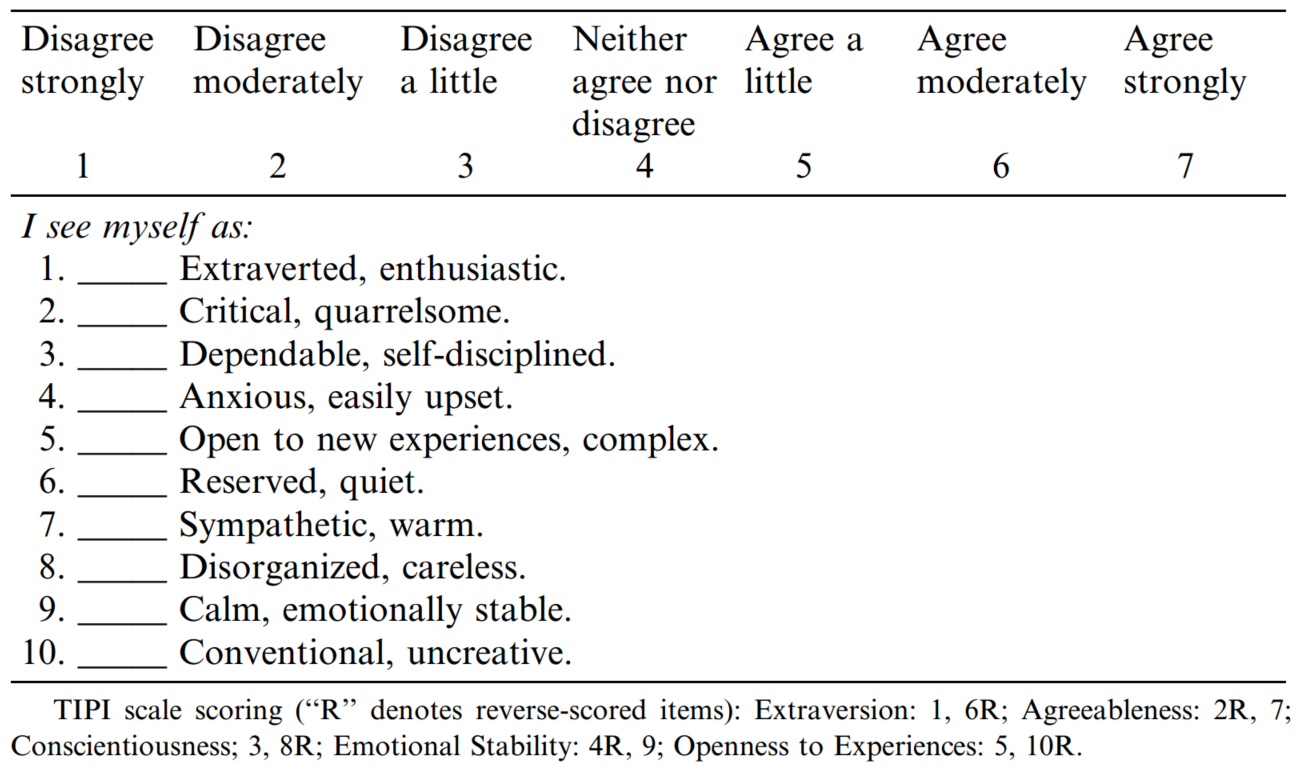
\includegraphics[width=.9\textwidth]{tipi.png}
\label{fig:tipi}
\fonte{\cite{gosling:03}}
\end{figure}

\section{Procedimento}
\label{sec:procedimento}

O procedimento do estudo de validação pode ser descrito em três passos, conforme ilustrado na Figura \ref{fig:estudo}.

No primeiro passo, aplicamos as métricas que detalhamos na Seção \ref{sec:metrics} para cada participante, utilizando a base de dados do Huxley. O período que consideramos para a coleta dos dados inicia-se na data de cadastro do usuário. A partir dessa data, analisamos a participação do mesmo, segundo a Tabela \ref{tab:dadosmetricas}, durante seis meses de uso do sistema. Esse período foi definido de acordo com o tempo do curso de Programação 1, período no qual os usuários mais utilizam o Huxley.%, que é de um semestre.

\begin{figure}[ht]
\centering
\caption{\small Procedimento do estudo de validação} 
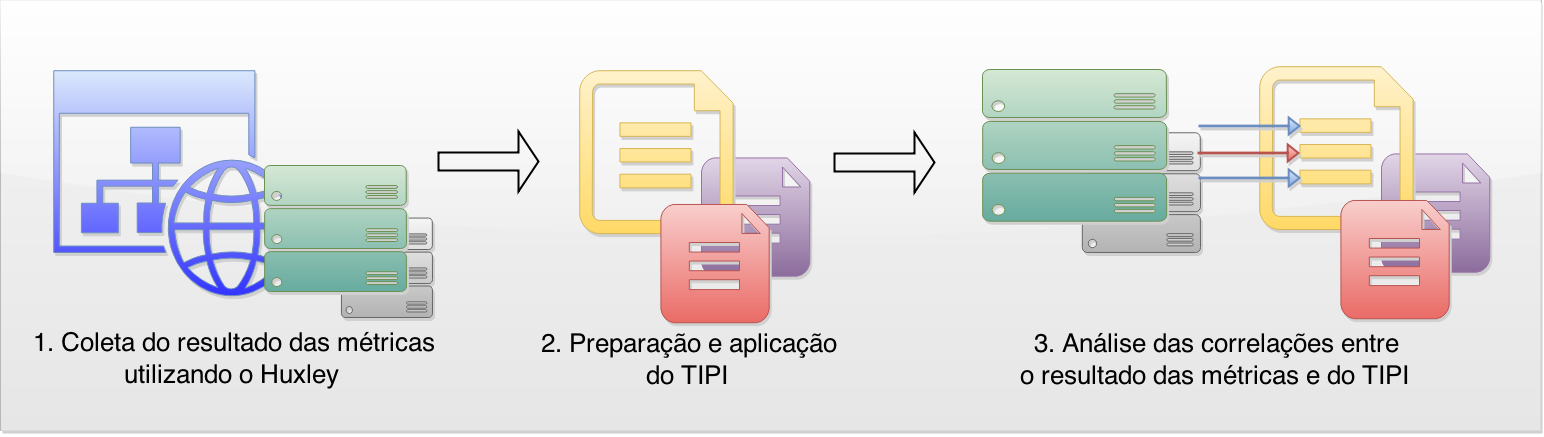
\includegraphics[width=.99\textwidth]{estudo.png}
\label{fig:estudo}
\end{figure}

Em seguida, no passo 2, preparamos o questionário TIPI para aplicá-lo ao grupo de participantes. O TIPI foi traduzido para Português buscando-se manter o significado de cada item. Apesar de alguns desses itens não estarem relacionados com as soft skills, não os removemos do questionário. Dessa forma, o apresentamos completo para avaliação dos participantes, mantendo-o o mais próximo possível de seu original para não comprometer a consistência dos itens.
%Além disso, disponibilizamos um link para acesso do TIPI em Inglês, caso o participante achasse necessário.

A fim de esclarecer o objetivo do questionário, também foram adicionadas informações contextuais aos itens. Essas informações adicionais tratam-se de frases curtas que permitem ao participante entender que suas respostas devem ser dadas de acordo com seu comportamento enquanto pratica atividades de programação. Como recomendado por John e Srivastava (1999)\nocite{john:99}, adicionar esclarecimentos ou informações contextuais em instrumentos curtos é importante para evitar problemas de mal-entendimento, como ambiguidade ou significados múltiplos.
O Apêndice \ref{ap:tipi} apresenta o instrumento que aplicamos durante este estudo de validação, nele pode-se ler os itens do TIPI e as informações contextuais que adicionamos.

O questionário TIPI foi aplicado presencialmente e individualmente para os participantes do estudo. No momento da aplicação, esclarecemos aos estudantes que suas participações não eram obrigatórias. Informamos também que suas identidades não seriam divulgadas, garantindo o anonimato das respostas, de forma que eles se sentissem à vontade para responder as questões de forma sincera.

A aplicação do TIPI ocorreu na última semana de aulas das disciplinas de Programação 1, ou seja, no mesmo período de tempo que as métricas das soft skills foram coletadas, no final do semestre. Nem todos os participantes estavam presentes, apenas 32 deles responderam o questionário. Em geral, nessa fase final da disciplina, os estudantes estão em menor número, pois muitos deixam de ir para as aulas ou mesmo desistem. Apesar de coletarmos as métricas para todos os matriculados, apenas os dados dos que responderam o questionário TIPI participam da verificação dos resultados.
%Mesmo porque, não faz sentido considerar soft skills de programador daqueles que nem sequer finalizaram a disciplina.

Então, para atingir o objetivo deste estudo, verificamos se os resultados que encontramos aplicando as métricas correspondem aos resultados do questionário, constituindo o passo 3.
Para isso, estamos considerando o coeficiente de correlação de Pearson entre as pontuações das soft skills e pontuações do teste de personalidade.
Baseamos este estudo, na relação que existe entre as soft skills e os fatores de personalidade que discutimos no Capítulo \ref{chap:concepts}.

Nossa hipótese é a seguinte: Uma métrica para identificação de soft skill pode ser validada se a mesma avalia sua respectiva soft skill em um nível que condiz com os traços de personalidade do indivíduo. Isso porque, se o indivíduo possui um determinado traço de personalidade, ele tende a possuir as soft skills relacionados a esse traço.

\section{Ameaças}
\label{sec:ameacas}

Algumas ameaças devem ser consideradas com relação a este estudo de validação, bem como precisamos discutir maneiras de contorná-las.
Inicialmente, sabemos que o fato de o questionário TIPI ser aplicado como um instrumento de auto avaliação pode levar a algum participante não o responder sinceramente. Isso pode acontecer porque alguém pode não se sentir à vontade de falar sobre si mesmo, e ainda, em nosso contexto onde os participantes são alunos, os mesmos podem ter receio de responder alguma declaração de forma negativa e dar conhecimento a seu professor de Programação.

Para lidar com esses possíveis problemas, consideramos analisar a consistência das respostas de cada participante. Para isso, calculamos as correlações dos itens do TIPI entre si. Os itens estão organizados em pares, de forma que, para cada fator do FFM existe um item positivo e um negativo. Por exemplo, o item \textit{1. Extrovertido, entusiasmado} indica o traço positivo do fator Extroversão. Já o item \textit{6. Reservado, quieto} é o traço negativo, ou inverso, indicando Introversão. Dessa forma, se um item do TIPI expressa uma declaração oposta a outro item, é preciso identificar uma correlação negativa entre os mesmos. Essa correlação deve assegurar a consistência das respostas.

Além disso, a fim de garantir que os participantes respondessem o questionário livremente, como já explicado na Seção \ref{sec:procedimento} sobre o procedimento, fizemos os estudantes cientes de que suas participações neste estudo eram opcionais e que seus dados não seriam expostos com identificação.

Outra ameaça considerada é a possibilidade de o participante não entender o questionário, ou não interpretar corretamente alguma declaração. Por esse motivo, traduzimos o questionário TIPI para o idioma Português com o cuidado de manter o instrumento o mais próximo possível de seu original. Também adicionamos informações contextuais para auxiliar os participantes a entenderem o contexto do questionário. Além de optarmos pela aplicação presencial, de forma que nos disponibilizamos a retirar qualquer dúvida no momento da coleta das respostas.

Durante as fases do estudo de validação, buscamos aplicar essas estratégias para contornar as possíveis ameaças e com a execução do mesmo fomos capazes de recolher dados suficientes para analisar os resultados desta pesquisa. A seguir, o Capítulo \ref{chap:results} vai tratar desses resultados.



%7%%7%%7%%7%%7%%7%%7%%7%%7%%7%%7%%7%%7%%7%%7%%7%%7%%7%%7
%                     Resultados                       %
%7%%7%%7%%7%%7%%7%%7%%7%%7%%7%%7%%7%%7%%7%%7%%7%%7%%7%%7

\chapter{Resultados}

\label{chap:results}

Neste capítulo apresentamos os resultados do estudo de validação descrito no capítulo \ref{chap:evaluation}. Inicialmente, na seção \ref{sec:tipitipi} discutimos a correlação entre os itens do questionário TIPI a fim de analisar a consistência das respostas dos participantes do estudo. Na seção \ref{sec:tipiss}, mostramos as correlações encontradas entre as respostas do TIPI e os valores das métricas para identificação de soft skills. Em seguida, discutimos os resultados na seção \ref{sec:discussao}.

\section{Correlações entre os itens do TIPI}
\label{sec:tipitipi}

De acordo com a proposta de Gosling et al. \cite{gosling:03}, os itens do TIPI denotam os cinco grandes fatores de personalidade (Big Five). Os itens estão organizados em pares, de forma que,
para cada fator existe um item positivo e um negativo.
Por exemplo, o item \textit{1. Extrovertido, entusiasmado} indica o traço positivo do fator Extroversão. Já o item \textit{6. Reservado, quieto} é o traço negativo, ou inverso, indicando Introversão.
Similarmente, a relação que existe entre os demais fatores e os itens é:
Amabilidade: \textit{2. Crítico, briguento} (negativo) e \textit{7. Compreensível, amável}; 
Conscienciosidade: \textit{3. Seguro, auto-disciplinado} e \textit{8. Desorganizado, descuidado} (negativo);
Neuroticismo: \textit{4. Ansioso, facilmente chateado} e \textit{9. Calmo, emocionalmente estável} (negativo);
Abertura à experiência: \textit{5. Aberto a novas experiências, complexo} e \textit{10. Convencional, não criativo} (negativo).

Quando um indivíduo responde o TIPI, ele auto-avalia sua personalidade pontuando os itens numa escala de 1 a 7, significando o valor 1 discordo fortemente, e 7, concordo fortemente.
Com isso, podemos entender que quanto maior for o valor escolhido para itens relativos ao traço positivo, menor será o valor respondido em itens dos respectivos traços negativos, e vice-versa.
Assim, para que haja consistência nas respostas do TIPI, precisamos encontrar uma correlação negativa entre os pares de itens:

\begin{itemize}
\item 1. Extrovertido, entusiasmado vs. 6. Reservado, quieto;
\item 2. Crítico, briguento vs. 7. Compreensível, amável;
\item 3. Seguro, auto-disciplinado vs. 8. Desorganizado, descuidado;
\item 4. Ansioso, facilmente chateado vs. 9. Calmo, emocionalmente estável;
\item 5. Aberto a novas experiências, complexo vs. 10. Convencional, não criativo.
\end{itemize}

Depois de coletar as respostas do questionário dos 32 participantes (total da amostra, N = 32),
examinamos as correlações dos 10 itens do TIPI entre si.
Fazemos isso a fim de analisar a consistência das respostas dos participantes. Observe a Tabela \ref{tab:tipitipi}.
Note que destacamos as correlações entre os itens do TIPI que são inversos. 

\begin{sidewaystable}[ph!]
\footnotesize
\caption{\small Correlação entre os itens do TIPI}
\addtolength{\tabcolsep}{1pt}
%\renewcommand{\arraystretch}{1.7} 
\centering

    \begin{tabular}{lcccccccccc}
    \toprule
          & \multicolumn{10}{c}{\textbf{Item}} \\
    \multicolumn{1}{c}{\textbf{Item}} & \textbf{1} & \textbf{6} & \textbf{2} & \textbf{7} & \textbf{3} & \textbf{8} & \textbf{4} & \textbf{9} & \textbf{5} & \textbf{10} \\
		\midrule
    \multicolumn{1}{l}{\textbf{1. Extrovertido, entusiasmado}} 						& -     &       &       &       &       &       &       &       &       &  \\
    \multicolumn{1}{l}{\textbf{6. Reservado, quieto}} 										& \textbf{-.29}	& -     &       &       &       &       &       &       &       &  \\
    \textbf{} & & & & & & & & & &  \\
    \multicolumn{1}{l}{\textbf{2. Crítico, briguento}} 										& -.25  & .11   & -     &       &       &       &       &       &       &  \\
    \multicolumn{1}{l}{\textbf{7. Compreensível, amável}} 								& .17   & -.39  & \textbf{-.48} & -     &       &       &       &       &       &  \\
    \textbf{} & & & & & & & & & &  \\
    \multicolumn{1}{l}{\textbf{3. Seguro, auto-disciplinado}} 						& .03   & -.14  & .22   & .04   & -     &       &       &       &       &  \\
    \multicolumn{1}{l}{\textbf{8. Desorganizado, descuidado}} 						& -.10  & -.01  & -.16  & .18   & \textbf{-.31} & -     &       &       &       &  \\
    \textbf{} & & & & & & & & & &  \\
    \multicolumn{1}{l}{\textbf{4. Ansioso, facilmente chateado}} 					& -.05  & -.03  & .44   & -.18  & .23   & -.05  & -     &       &       &  \\
    \multicolumn{1}{l}{\textbf{9. Calmo, emocionalmente estável}} 				& .08   & -.01  & -.31  & .18   & -.12  & .24   & \textbf{-.59} & -     &       &  \\
    \textbf{} & & & & & & & & & &  \\
    \multicolumn{1}{l}{\textbf{5. Aberto a novas experiências, complexo}} & .16   & -.27  & -.34  & .28   & .17   & .06   & -.07  & .24   & -     &  \\
    \multicolumn{1}{l}{\textbf{10. Convencional, não criativo}} 					& -.44  & .25   & .08   & -.26  & -.07  & .09   & -.10  & .04   & \textbf{.07} & - \\
    
		\bottomrule
		\textbf{} & & & & & & & & & &  \\
		\textit{Nota: N = 32} & & & & & & & & & &  \\
		
%\begin{tabular}{|lcccccccccc|}
%\hline
%							& \multicolumn{10}{c|}{\textbf{Item}}	 				\\ \hline
%\textbf{Item} & 1 & 2 & 3 & 4 & 5 & 6 & 7 & 8 & 9 & 10 		\\ \hline \hline 

%1. Extrovertido, entusiasmado						& $-$ 	 				&      &       					&       &  		 					& 		  &		   					&		   &  		 				 &  		\\ \hline 
%6. Reservado, quieto											& \textbf{-.29} & $-$  &       					&       &  		 					& 		  &		   					&		   &  		 				 &  		\\ \hline \hline 

%2. Crítico, briguento										& $-.25$ 				& .11  & $-$  					&       &  		 					& 		  &		   					&		   &  		 				 &  		\\ \hline 
%7. Compreensível, amável									& $.17$  				& -.39 & \textbf{-.48}  & $-$   &      					&  		  & 							&		   &  		 				 &  		\\ \hline \hline 
 
%3. Seguro, auto-disciplinado							& $.03$  				& -.14 &  .22  					& .04	  & $-$  					&  		  &  		 					& 		 &  		 				 &  		\\ \hline 
%8. Desorganizado, descuidado							& $-.10$ 				& -.01 & -.16  					& .18	  & \textbf{-.31} & $-$   & 		 					&  		 &  		 				 &  		\\ \hline \hline 
 
%4. Ansioso, facilmente chateado					& $-.05$ 				& -.03 &  .44  					& -.18  &  .23 					& -.05	& $-$  					&  		 &  		 				 &  		\\ \hline 
%9. Calmo, emocionalmente estável					&  $.08$ 				& -.01 & -.31  					&  .18	& -.12 					&  .24	& \textbf{-.59} & $-$  &  		 				 &  		\\ \hline \hline 

%5. Aberto a novas experiências, complexo	& $.16$  				& -.27 & -.34  					&  .28	&  .17 					&  .06	& -.07 					&  .24	& $-$  				 &  		\\ \hline 
%10. Convencional, não criativo						& $-.44$ 				&  .25 &  .08  					& -.26	& -.07 					&  .09	& -.10 					&  .04	& \textbf{.07} & $-$  \\ \hline 

\end{tabular}
\label{tab:tipitipi}
\end{sidewaystable}

Somente para o fator Abertura à experiência, a correlação entre os itens \textit{5. Aberto a novas experiências, complexo} e \textit{10. Convencional, não criativo} não é negativa e é muito próxima a 0. Isso indica que pode haver inconsistência nas respostas dadas para os itens relativos a esse fator.
É importante considerar essa informação, pois esse problema pode afetar também as correlações entre os mesmos itens e as métricas que aplicamos.
%Isso porque, as respostas desses itens no questionário não são totalmente confiáveis.
%portanto, isso pode gerar incoonsistência também quando analisamos sua correlação com os resultados das métricas que aplicamos.

Essa inconsistência pode ter ocorrido porque os participantes não entenderam os itens e/ou por limitações do próprio instrumento. Gosling et al. \cite{gosling:03}, apresentam uma tabela similar em seu artigo. A correlação entre os itens do fator Abertura à experiência é, relativamente, a menos significativa (-.28, N = 1799, p> .05).
Nas demais dimensões, as correlações são: Amabilidade: -.36; Conscienciosidade: -.42; Extroversão: -.59; e Neuroticismo: -.61, (N = 1799, p> .05).
%É possível que a mudança de idioma tenha afetado a qualidade dos itens.

\section{Correlações entre as métricas e os itens do TIPI}
\label{sec:tipiss}

Examinamos as correlações entre as pontuações obtidas a partir das métricas para identificação das soft skills e os itens do TIPI a fim de verificar como as métricas estão relacionadas com os fatores de personalidade. A relação que estamos procurando foi discutida no capítulo \ref{chap:concepts} e sumarizada na Figura \ref{fig:mapeamento}.
Podemos observar as correlações obtidas na Tabela \ref{tab:tipiss}. Note que destacamos as correlações esperadas. 

\begin{sidewaystable}[ph!]
\footnotesize
\caption{\small Correlações entre as métricas e os itens do TIPI}
\addtolength{\tabcolsep}{1pt}
%\renewcommand{\arraystretch}{1.7} 
\centering
\begin{tabular}{lccccc}

    \toprule		
		& \textbf{1. Extrovertido, }  & \textbf{2. Crítico, } & \textbf{3. Seguro, } 			 & \textbf{4. Ansioso, } 				& \textbf{5. Aberto a novas } \\
		& \textbf{entusiasmado} 			& \textbf{briguento} 		& \textbf{auto-disciplinado} & \textbf{facilmente chateado} & \textbf{experiências, complexo} \\
					
    \midrule
    \multicolumn{1}{c}{\textbf{Análise de problemas}} 		& .353  				 & -.250 & \textbf{.337} & .080  & .203 				 \\
    \multicolumn{1}{c}{\textbf{Resolução de problemas}}		& -.198  				 & .143  & \textbf{.416} & .169  & .291 				 \\
    \multicolumn{1}{c}{\textbf{Atenção a detalhes}} 			& .243  				 & -.035 & \textbf{.343} & .365  & .171 				 \\
    \multicolumn{1}{c}{\textbf{Aprendizagem rápida}} 			& -.050  				 & -.136 & \textbf{.393} & .040  & \textbf{.307} \\
    \multicolumn{1}{c}{\textbf{Persistência}} 						& -.080  				 & .087  & \textbf{.307} & -.010 & .178 				 \\
    \multicolumn{1}{c}{\textbf{Comunicação}} 							& \textbf{-.163} & .200  & .134  			   & -.076 & -.117 				 \\
    \multicolumn{1}{c}{\textbf{Trabalho independente}} 		& .030  				 & -.142 & -.064 				 & -.026 & -.026 				 \\ 
		
    \multicolumn{1}{c}{\textbf{}} & & & & &  \\
		
    \toprule
		& \textbf{6. Reservado, } & \textbf{7. Compreensível, } & \textbf{8. Desorganizado, } & \textbf{9. Calmo, } 						& \textbf{10. Convencional, } \\
		& \textbf{quieto} 				& \textbf{amável} 						& \textbf{descuidado}					& \textbf{emocionalmente estável} & \textbf{não criativo} \\ 
		
		\midrule
    \multicolumn{1}{c}{\textbf{Análise de problemas}} 		& -.257 				 & \textbf{.209}  & .038  & .114  & -.266 				 \\
    \multicolumn{1}{c}{\textbf{Resolução de problemas}} 	& -.178 				 & \textbf{-.042} & .138  & -.147 & .163 				   \\
    \multicolumn{1}{c}{\textbf{Atenção a detalhes}} 			& -.305 				 & .107 				  & -.011 & -.180 & \textbf{-.222} \\
    \multicolumn{1}{c}{\textbf{Aprendizagem rápida}} 			& -.165 				 & .018 				  & .308  & .058  & -.076  				 \\
    \multicolumn{1}{c}{\textbf{Persistência}} 					  & -.263 				 & .024 				  & .013  & -.077 & -.025 				 \\
    \multicolumn{1}{c}{\textbf{Comunicação}} 							& .030 				   & -.025 				  & .158  & -.009 & -.141 				 \\
    \multicolumn{1}{c}{\textbf{Trabalho independente}} 		& \textbf{.183}  & .073 				  & .229  & -.189 & .035 				   \\
    
		\bottomrule
		\multicolumn{1}{l}{\textbf{}} & & & & &  \\
		\multicolumn{1}{l}{\textit{Nota: N = 32}} & & & & &  \\
		
\end{tabular}
\label{tab:tipiss}
\end{sidewaystable}

\section{Discussão}
\label{sec:discussao}

Esperava-se que as métricas Análise de problemas e Resolução de problemas apresentassem correlações positivas com os itens \textit{3. Seguro, auto-disciplinado} e \textit{7. Compreensível, amável}. Encontramos resultados positivos para o fator de Conscienciosidade (.337 e .416). Quanto ao fator Amabilidade, a correlação positiva ocorre com a métrica Análise de problemas (.209). Apesar de não esperada, também encontramos correlação entre a métrica Análise de problemas e o item \textit{1. Extrovertido, entusiasmado }(.353).

As métricas Atenção a detalhes, Aprendizagem rápida e Persistência também mostram correlação positiva (.343, .393, e .307, respectivamente) com o item esperado, \textit{3. Seguro, auto-disciplinado}. Esse resultado indica que essas métricas identificam as soft skills relacionadas com fator Conscienciosidade.

Aprendizagem rápida e o item \textit{5. Aberto a novas experiências, complexo}, apresentam correlação positiva (.307), como esperado. Com isso, é possível observar que a métrica está associada com características de um indivíduo aberto a novas experiências e que aprecia aprender coisas novas. A métrica Trabalho independente também mostrou correlação positiva (.183) com o item esperado, \textit{6. Reservado, quieto}.

\subsection{Correlações inversas ou insignificantes}

Existem correlações esperadas que não fomos capazes de encontrar. A correlação entre a métrica Resolução de problemas e o item \textit{7. Compreensível, amável} é insignificante. É possível que não encontramos essa correlação porque a métrica apenas engloba traços de seu outro fator relacionado, Conscienciosidade, não apresentando características de Amabilidade. Sabemos que este fator é uma dimensão da personalidade sobre interação interpessoal, por outro lado, a métrica foi aplicada em um sistema virtual onde não há recursos de interação social. Isso também pode explicar porque a métrica Análise de problemas e o mesmo item têm uma correlação positiva, mas baixa.

A métrica Atenção a detalhes mostra uma correlação negativa com o item
%que representa o traço inverso de Abertura à experiência,
\textit{10. Convencional, não criativo}, no entanto, esperava-se uma correlação positiva.
%, que representa o fator Abertura a experiência de forma negativa.
Nesse caso, nos remetemos à inconsistência entre os itens do TIPI referentes a esse fator, como mencionado na seção \ref{sec:tipitipi}.
%onde identificamos correlação insignificante.
Esse pode ser o motivo de termos identificado essa correlação de maneira inversa.
Com isso, não podemos afirmar se a métrica está ou não correlacionada com o traço de personalidade esperado.

Apesar de esperarmos correlação positiva, a métrica Comunicação apresenta correlação negativa com o item \textit{1. Extrovertido, entusiasmado}.
%Entendemos que, uma vez que a métrica apenas considera comentários em códigos-fonte para identificar a soft skill, então ela só está identificando habilidades de comunicação escrita. Assim, podemos também considerar traços de introversão. No entanto, a métrica tem correlação insignificante com a característica inversa de extroversão, \textit{6. Reservado, quieto}.
Essa métrica não apresenta resultados satisfatórios possivelmente porque utiliza poucos recursos para identificação da soft skill,
uma vez que apenas considera comentários em códigos-fonte para identificar habilidades de comunicação,
por falta de funcionalidades como bate-papo ou fórum no Huxley.
%Assim, não podemos dizer por meio dessa métrica se um indivíduo tem habilidades de comunicação.

\subsection{Significância das correlações}

Para saber se os nossos resultados podem ser aplicados em uma população geral, precisamos aplicar inferência e analisar além dos nossos dados
%, uma vez que o tamanho da amostra de estudo foi de apenas 32.
Nesta subseção estamos mostrando os valores de \textit{p} para cada correlação esperada entre métricas e os itens do questionário TIPI.
Com \textit{p-value}, somos capazes de reconhecer se os resultados encontrados não foram produzidos por dados aleatórios.
A Tabela \ref{tab:pvalue} resume as correlações encontradas e adiciona a informação \textit{p-value}.

\begin{sidewaystable}[ph!]
\footnotesize
\caption{\small Correlações entre as métricas e os itens do TIPI, p-value}
\addtolength{\tabcolsep}{1pt}
%\renewcommand{\arraystretch}{1.7} 
\centering
\begin{tabular}{lccc}

    \toprule
          & \textbf{1. Extrovertido, entusiasmado} & \textbf{3. Seguro, auto-disciplinado} & \textbf{5. Aberto a novas experiências, complexo} \\
    \midrule
    \multicolumn{1}{c}{\textbf{Análise de problemas}} 	& \textbf{0.353; p = .04} & \textbf{0.337; p = .06} & \textbf{} \\
    \multicolumn{1}{c}{\textbf{Resolução de problemas}} &													& \textbf{0.416; p = .02} & \textbf{} \\
    \multicolumn{1}{c}{\textbf{Atenção a detalhes}} 		&													& \textbf{0.343; p = .05} &  \\
    \multicolumn{1}{c}{\textbf{Aprendizagem rápida}} 		&													& \textbf{0.393; p = .02} & \textbf{0.307; p = .09} \\
    \multicolumn{1}{c}{\textbf{Persistência}} 					&													& \textbf{0.307; p = .08} &  \\
    \multicolumn{1}{c}{\textbf{Comunicação}} 						& -0.163; p = .37					&													&  \\
    \multicolumn{1}{c}{\textbf{Trabalho independente}} 	&													&													&  \\
		
          &  &  &  \\

		\toprule					
          & \textbf{6. Reservado, quieto} & \textbf{7. Compreensível, amável} & \textbf{10. Calmo, emocionalmente estável} \\
		\midrule			
    \multicolumn{1}{c}{\textbf{Análise de problemas}} 	&													& 0.209; p = .25 	&  \\
    \multicolumn{1}{c}{\textbf{Resolução de problemas}} &													& -0.042; p = .82 &  \\
    \multicolumn{1}{c}{\textbf{Atenção a detalhes}} 		&													&       					& -0.222; p = .22 \\
    \multicolumn{1}{c}{\textbf{Aprendizagem rápida}} 		&													&       					&  \\
    \multicolumn{1}{c}{\textbf{Persistência}} 					&													&       					&  \\
    \multicolumn{1}{c}{\textbf{Comunicação}} 						&													&       					&  \\
    \multicolumn{1}{c}{\textbf{Trabalho independente}}	& 0.183; p = .31 					&									&  \\
		
    \bottomrule
		\multicolumn{1}{l}{\textbf{}} & & & \\
		\multicolumn{1}{l}{\textit{Nota: N = 32}} & & & \\
    
		
\end{tabular}
\label{tab:pvalue}
\end{sidewaystable}

Note que a Tabela \ref{tab:pvalue} mostra os mesmos valores de correlação da Tabela \ref{tab:tipiss}. 
As células vazias e colunas ocultas são valores insignificantes e/ou que não precisamos considerar.
%por conta da falta de relacionamento entre as soft skills e os fatores de personalidade. ? Não é bem isso...
Apenas mostramos as correlações que esperamos, de acordo com as associações que existem entre as soft skills e os fatores de personalidade.
%Também observamos a correlação entre a métrica Análise de problemas e item \textit{1. Extrovertido, entusiasmado}.
Em destaque, apresentamos as correlações significativas, considerando \textit{p-value} inferior a 0,1 (N = 32; p < .1).


%8%%8%%8%%8%%8%%8%%8%%8%%8%%8%%8%%8%%8%%8%%8%%8%%8%%8%%8
%                      Conclusão                       %
%8%%8%%8%%8%%8%%8%%8%%8%%8%%8%%8%%8%%8%%8%%8%%8%%8%%8%%8

\chapter{Conclusão}

\label{chap:conclusion}

Durante esta pesquisa, abordamos a relevância e a aplicação das soft skills para a qualificação de um profissional. Com foco no papel do programador, profissão da área de desenvolvimento de software e de Tecnologia da Informação, fizemos o levantamento de importantes soft skills que o respectivo setor de trabalho exige. Destacamos as soft skills Análise e resolução de problemas, Atenção a detalhes, Aprendizagem rápida, Persistência, Comunicação e Trabalho independente como habilidades diferenciais para integração, permanência e crescimento do programador como profissional.

Através de conceitos provenientes de teorias sobre personalidade, como o Modelo dos Cinco Fatores (FFM), buscamos esclarecer o significado de cada soft skill em destaque, aprendendo as características e comportamento dos indivíduos que as possuem. Discutimos também o motivo pelo qual elas são importantes para o programador de software e como aplicam-se no contexto dessa profissão. Assim, construímos uma base teórica e conceitual para o desenvolvimento de uma estratégia que visa oferecer uma alternativa para identificação de soft skills em programadores, utilizando-se de uma abordagem automática.

Nossa estratégia propõe um conjunto de sete métricas que pontuam o nível das soft skills que um indivíduo possui. As métricas são aplicadas a um sistema de programação online chamado Huxley, categorizado como juiz online. A partir da base de dados do Huxley, coletamos essas métricas e elaboramos um estudo empírico para validação das mesmas. Esse estudo também utiliza-se do FFM, através de um questionário a respeito de personalidade chamado TIPI (Ten-Item Personality Inventory). Os participantes do estudo, como usuários do Huxley, foram avaliados diante das métricas que identificam suas soft skills. Os mesmos também responderam o TIPI e comparamos os resultados em busca de analisar se as métricas das soft skills condizem com os traços de personalidades.

De acordo com os resultados de nosso estudo de validação, as métricas Comunicação e Trabalho independente não mostram resultados relevantes. Suas correlações com os traços de personalidades esperados não são significantes. Sendo assim, indicamos que essas métricas necessitam ser revistas e aprimoradas. Não aconselhamos a utilização das mesmas para identificação automática de soft skills.

Por outro lado, podemos indicar cinco métricas que funcionam de maneira satisfatória, são elas: Análise de problemas, Resolução de problemas, Atenção a detalhes, Aprendizagem rápida e Persistência. Essas métricas apresentam correlações significantes com os traços de personalidade associados à suas respectivas soft skills.
Portanto, elas podem ser utilizadas para identificar se um programador possui alguma dessas habilidades. É importante observar, que cada métrica traz essa informação através de um valor entre zero e 100, significando que quanto maior o valor da métrica, maior o nível de desenvolvimento da soft skill. Dessa maneira, é possível perceber as habilidades que são pontos fortes de um indivíduo, como também aquelas que precisam de melhoria. O nível da habilidade também pode ser útil para ordenar um conjunto de candidatos a vagas de emprego, por exemplo.

Apesar de não ter sido possível validar todas as métricas, a maioria delas pode ser aplicada para identificação automática de soft skills. Com isso, consideramos que nossos objetivos foram atingidos. Em suma, esta dissertação traz diversas contribuições:

\begin{itemize}
 \item Ampliamos a compreensão sobre aspectos humanos relacionados ao desenvolvimento de software, chamando atenção para habilidades importantes, porém muitas vezes ignoradas ou não compreendidas; 

 \item Fizemos uma levantamento de importantes soft skills para o programador de software. Adicionalmente, apontamos o relacionamento das mesmas com teorias de personalidade e explicamos como elas se aplicam no contexto da profissão. Com isso, trazemos informações para o profissional, no reconhecimento das necessidades do ambiente de trabalho e na reflexão dos atributos que precisa desenvolver; para os educadores e aprendizes de programação, no processo de construção de suas habilidades; e para as empresas, no conhecimento das competências do profissional qualificado;
%e para as empresas podem utilizar as métricas como alternativa para identificar os profissionais que precisam contratar.

 \item Elaboramos uma estratégia automática para a identificação de soft skills, a partir do desenvolvimento de métricas. Também, descrevemos os passos de um estudo de validação para as mesmas, que originalmente as correlacionam com traços de personalidade.
Essa estratégia pode ser replicada em outros ambientes similares ao Huxley, onde as métricas propostas podem ser adaptadas, ou mesmo, onde novas métricas podem ser criadas e avaliadas seguindo os passos do estudo de validação;

 \item Desenvolvemos e validamos métricas para identificar automaticamente soft skills em programadores, oferecendo uma alternativa às empresas no processo de contratação de profissionais;
\end{itemize}

Como trabalhos futuros, propomos que as métricas validadas sejam implantadas no juiz online Huxley, constituindo uma nova funcionalidade de identificação de soft skills para o sistema. A página de perfil dos usuários pode exibir as principais habilidades de cada um, destacando-as através de ícones (como um selo ou conquista). Essa ideia pode incentivá-los a adquirir e desenvolver soft skills importantes.

Além disso, recomendamos a criação de uma página de busca de usuários por soft skills. Tal funcionalidade pode ser direcionada para empresas, de forma que o sistema os indicasse a empregos de programador, de acordo com suas habilidades mais desenvolvidas. No contexto do Huxley, isso é especialmente útil porque a maioria dos membros ainda são estudantes e não possuem experiência profissional. Portanto, eles não contam com recomendações de antigos empregos, mas poderiam utilizar as indicações do sistema como forma de demonstrar suas soft skills.

Aconselhamos também a implementação de funcionalidades como bate-papo, fóruns, grupos de estudos, comunidade de membros, etc., como forma de melhorar a interação entre os usuários do Huxley. Tais funcionalidades, além de incrementar o sistema, poderiam ser empregadas na melhoria da métrica Comunicação, por exemplo.

Tanto a referida métrica, quanto Trabalho independente, precisam ser revisadas. Propomos que pesquisas futuras sejam realizadas nesse sentido, sendo também possível trabalhar na melhoria das métricas que já demonstram aplicação.
%, a fim de atingir melhores níveis de correlação com os traços de personalidade associados.






%Fim dos elementos textuais
\postextual

\bibliography{bibliography}

\apendices

\chapter{Questionário para avaliação de soft skills do programador}
\label{ap:tipi}

%Você está prestes a responder um questionário que trata de personalidade e está voltado ao seu perfil como programador de software.
%Para começar, informe corretamente seu username e email no Huxley: 

%\begin{tabular}{lp{5cm}}
%Username no Huxley & \noindent\rule{5cm}{0.4pt} \\

%Email no Huxley	 	 & \noindent\rule{5cm}{0.4pt} \\
%\end{tabular}

\section{Contextualização}

Você está prestes a responder um questionário que trata de personalidade e está voltado ao seu perfil como programador de software.
Quando responder o questionário Ten-Item Personality Inventory - TIPI, imagine você mesmo quando está programando, ou seja, avalie seu comportamento em atividades relacionadas à programação. Observe que algumas questões contam com uma breve descrição que te ajudará a contextualizá-las. Seja sincero em suas respostas.

Se desejar consultar o questionário TIPI original (em Inglês), veja a página 22 do artigo de Gosling et al. (2003)\nocite{gosling:03}, em:
\href{http://goo.gl/ha6Zr4}{\textsl{http://goo.gl/ha6Zr4}}.

As respostas deste questionário contribuem para a pesquisa de mestrado da aluna Maria Helynne Lima Silva, sob orientação do professor Rodrigo de Barros Paes, do Programa de Pós-Graduação em Informática do Instituto de Computação da Universidade Federal de Alagoas.

\section{Ten-Item Personality Inventory – TIPI}

Aqui estão alguns traços de personalidade que podem ou não aplicar-se a você.  Por favor, escolha um número em cada declaração para indicar o quanto você concorda ou discorda com cada declaração. Você deve pontuar o quanto cada traço aplica-se a você, mesmo se uma característica aplica-se mais fortemente que a outra.

\vspace{0.5cm}
\noindent
\begin{tabular}{lll}
\footnotesize 1 – Discordo fortemente 		& 																						& \footnotesize 5 – Concordo um pouco\\
\footnotesize 2 – Discordo moderadamente 	& \footnotesize 4 – Nem concordo nem discordo	& \footnotesize 6 – Concordo moderadamente\\
\footnotesize 3 – Discordo um pouco 			&																							& \footnotesize 7 – Concordo fortemente\\
\end{tabular}

\vspace{0.5cm}
\textbf{Eu me vejo como:}
\vspace{0.5cm}

\noindent
\textbf{1. Extrovertido, entusiasmado} \footnotesize \textsl{- Em relação a ser comunicativo}
\normalsize
 
\begin{figure}[!h]
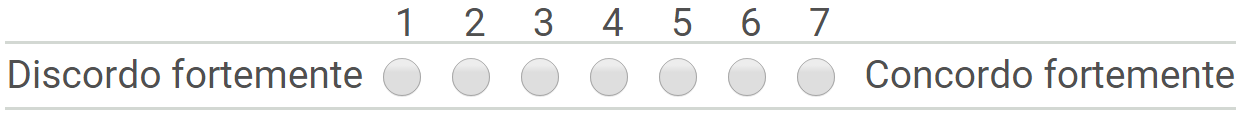
\includegraphics[width=.65\textwidth]{likert.png}
\end{figure}

\newpage%
\noindent
\textbf{2. Crítico, briguento}

\begin{figure}[!h]
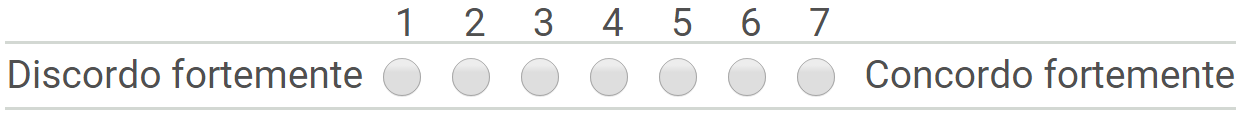
\includegraphics[width=.65\textwidth]{likert.png}
\end{figure}

\noindent  
\textbf{3. Seguro, autodisciplinado}   \footnotesize \textsl{- Em relação a executar suas tarefas com persistência}
\normalsize

\begin{figure}[!h]
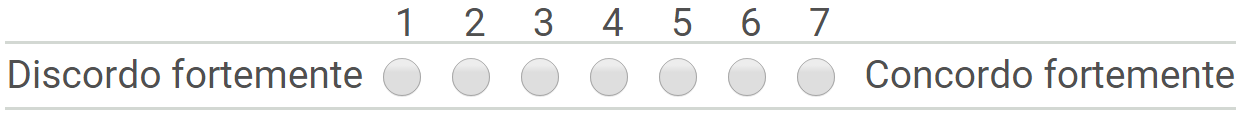
\includegraphics[width=.65\textwidth]{likert.png}
\end{figure}
 
\noindent
\textbf{4. Ansioso, facilmente chateado}

\begin{figure}[!h]
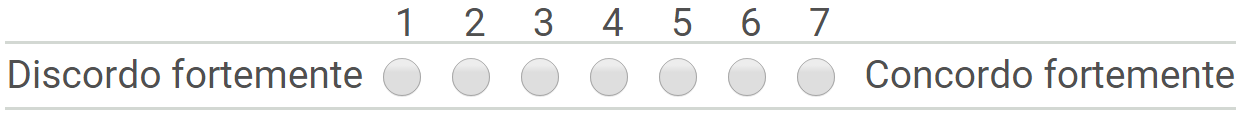
\includegraphics[width=.65\textwidth]{likert.png}
\end{figure}

\noindent
\textbf{5. Aberto a novas experiências, complexo} 

\begin{figure}[!h]
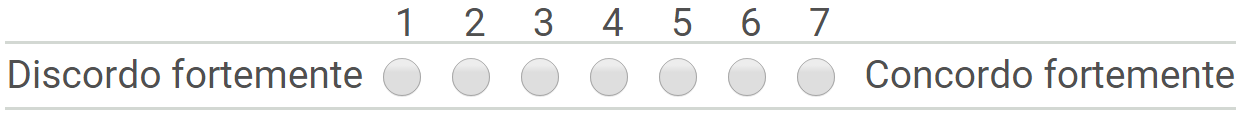
\includegraphics[width=.65\textwidth]{likert.png}
\end{figure}
 
\noindent
\textbf{6. Reservado, quieto}          \footnotesize \textsl{- Em relação a pedir ajuda de outras pessoas} \normalsize

\begin{figure}[!h]
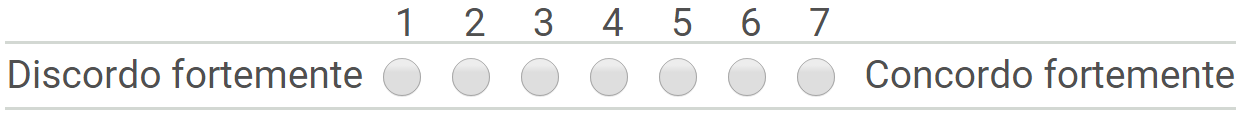
\includegraphics[width=.65\textwidth]{likert.png}
\end{figure}
 
\noindent
\textbf{7. Compreensivo, amável}       \footnotesize \textsl{- Em relação à forma como lida com as pessoas}\normalsize

\begin{figure}[!h]
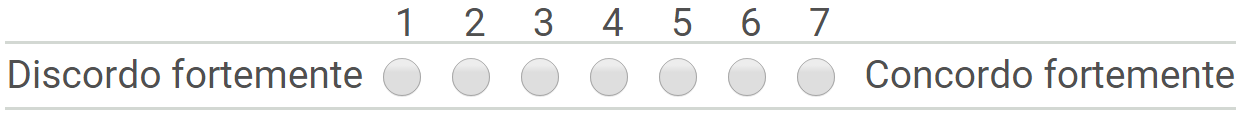
\includegraphics[width=.65\textwidth]{likert.png}
\end{figure}

\noindent
\textbf{8. Desorganizado, descuidado}

\begin{figure}[!h]
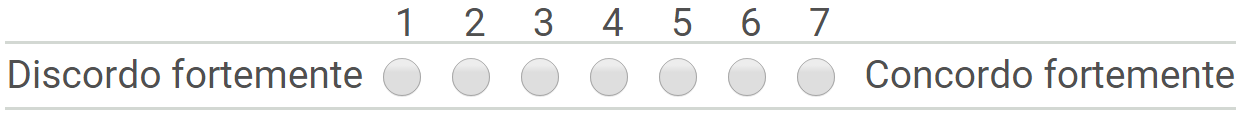
\includegraphics[width=.65\textwidth]{likert.png}
\end{figure}
 
\noindent
\textbf{9. Calmo, emocionalmente estável}

\begin{figure}[!h]
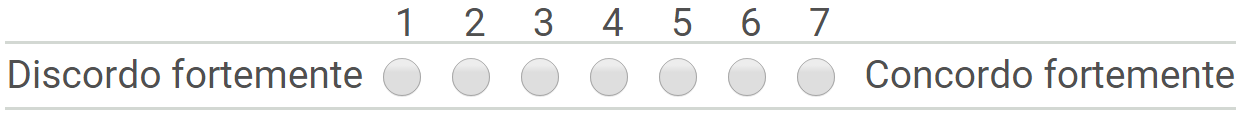
\includegraphics[width=.65\textwidth]{likert.png}
\end{figure}
 
\noindent
\textbf{10. Convencional, não criativo}  

\begin{figure}[!h]
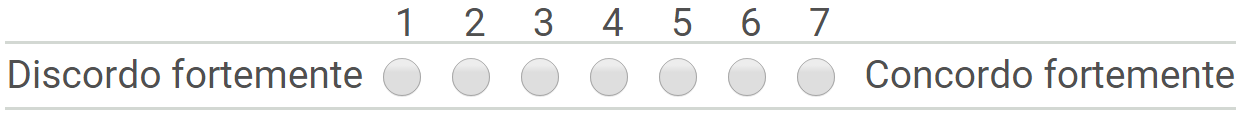
\includegraphics[width=.65\textwidth]{likert.png}
\end{figure}



\end{document}

\pdfbookmark